%------------------------------- CHAPTER NAME --------------------------------
\chapter{High lift devices effects}
\label{chap:HighLift}

\begin{flushright}
	{\smaller
		\textit{There are two critical points in every aerial flight—its beginning and its end.}\\
		-- Alexander Graham Bell, 1906}
\end{flushright}

\noindent
In the preliminary design of the wing a large number of requirements have to be fulfilled as exemplified in table~\ref{table:WingRequirements}; but, as many of them are in conflict, it is hardly ever possible to check them all, so that a compromise has to be found.
%
\begin{table}[H]
\makebox[\linewidth]{
\begin{tabular}{l}
\toprule
High lift to drag ratio $L/D$ \\
Satisfactory maximum lift coefficient \\
Satisfactory stall quality \\
High value of the critical Mach number \\
Low weight \\
Ensure satisfactory performance in all flight phases \\
\bottomrule
\end{tabular}
}
\caption{Some wing design requirements}
\label{table:WingRequirements}
\end{table}

\noindent
With respect of the last shown requirement, the wing is usually equipped with high-lift devices, which change it's shape, in order to make it performing both in cruise both in take-off and landing phases. In fact, as can be seen from table~\ref{table:cruiseTOLand}, these phases show conflicting objectives which can only be mediated through the introduction of these devices.
%
\begin{table}[H]
\makebox[\linewidth]{
\begin{minipage}{0.5\textwidth}
\leftline{	
\begin{tabular}{l}
\toprule
\textbf{Cruise requirements} \\
\midrule
Small wing surface and high wing \\
loading $W/\!S$ \\ [0.1 cm] 
Small camber \\ [0.1 cm]
Low drag \\ [0.1 cm]
High speed \\ [0.1 cm]
Lift generated using low C\textsubscript{L} \\ 
\bottomrule
\end{tabular}
}
\end{minipage}
\begin{minipage}{0.5\textwidth}
\rightline{
\begin{tabular}{l}
\toprule
\textbf{Take-Off and Landing requirements} \\
\midrule
Big wing surface, or high C\textsubscript{Lmax}, in order \\
to have an high equivalent wing loading \\
$m=W/(\!S\cdot C_{L\text{max}})$ \\ [0.2 cm]
High drag value in landing \\ [0.2 cm]
Lift generated using high C\textsubscript{L} due to the \\
low speed \\ 
\bottomrule
\end{tabular}
}
\end{minipage}
}
\caption{Comparison between cruise and take-off/landing design requirements}
\label{table:cruiseTOLand}
\end{table}
%
%-------------------------- THEORETICAL BACKGROUND ---------------------------
\section{Theoretical background}
\label{sec:theoryFlapSlat}
In this paragraph, a general overview of the different type of high-lift devices is provided as well as the semi-empirical steps used to predict their effects on aerodynamic performance of the wing.

\bigskip
\noindent
The designer may choose from a large collection of feasible high-lift systems, although in the case of a specific project this freedom will be limited, since incremental drag, mechanical complexity, development and maintenance costs and structural weight are all factors to be considered~\cite{torenbeek1982synthesis}.

\bigskip
\noindent
All high-lift devices can be divided in two main groups of which only the first one will be analyzed in this discussion:
%
\begin{itemize}
\item Systems for passive lift increase, such as \emph{leading-edge devices} or \emph{trailing-edge devices}, which modify the wing shape.
\item Systems for active lift increase, such as \emph{blown flaps} or \emph{jet flaps}, which acts directly on the flow in order to control it.
\end{itemize}
%
\noindent
Generally speaking, \emph{trailing-edge devices} are used to increase the wing maximum lift coefficient, while \emph{leading-edge devices} are used to increase the stalling angle of attack. 
%
A more in depth analysis shows that \emph{trailing-edge devices} increase the camber and improve the flow at the trailing edge, but tend to promote leading edge stall on thin sections and may cause a reduction in the stalling angle of attack; on the other hand \emph{leading-edge devices} postpone or eliminate leading edge stall, but  they have little effects on the airfoil camber as a whole, although locally the camber is increased~\cite{torenbeek1982synthesis}.

\bigskip
\noindent
About \emph{trailing-edge devices}, their effects can be resumed in:
%
\begin{itemize}
\item Higher C\textsubscript{L} at a given angle of attack and higher C\textsubscript{Lmax}
\item Lower stalling angle of attack
\item Lower zero-lift angle due to increasing camber
\end{itemize}
%
\noindent
while \emph{leading-edge devices} provide the followings:
\begin{itemize}
\item Extension of the linear trait of the lift curve with an increase of the maximum angle of attack and of the C\textsubscript{Lmax}
\item Higher zero-lift angle due to translation of the lift curve on the right caused by leading edge deflection which reduce the actual angle of attack 
\item Higher slope of the linear trait of the lift curve, for those devices which extend airfoils chords with the effect of increase the wing surface and, with constant wing span, the aspect ratio
\end{itemize}
%
\begin{figure}
\centering
\begin{minipage}{.5\textwidth}
\centering
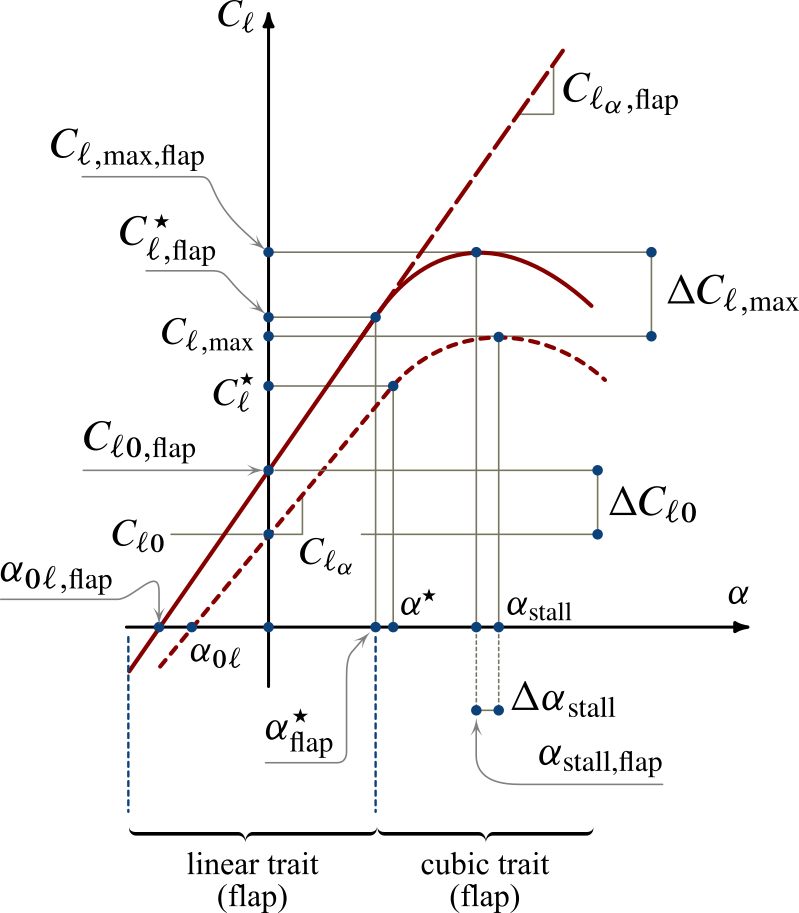
\includegraphics[width=.9\linewidth]{FlapEffects}
\captionof{figure}{Trailing-edge devices effects}
\label{fig:FlapEffects}
\end{minipage}%
\begin{minipage}{.5\textwidth}
\centering
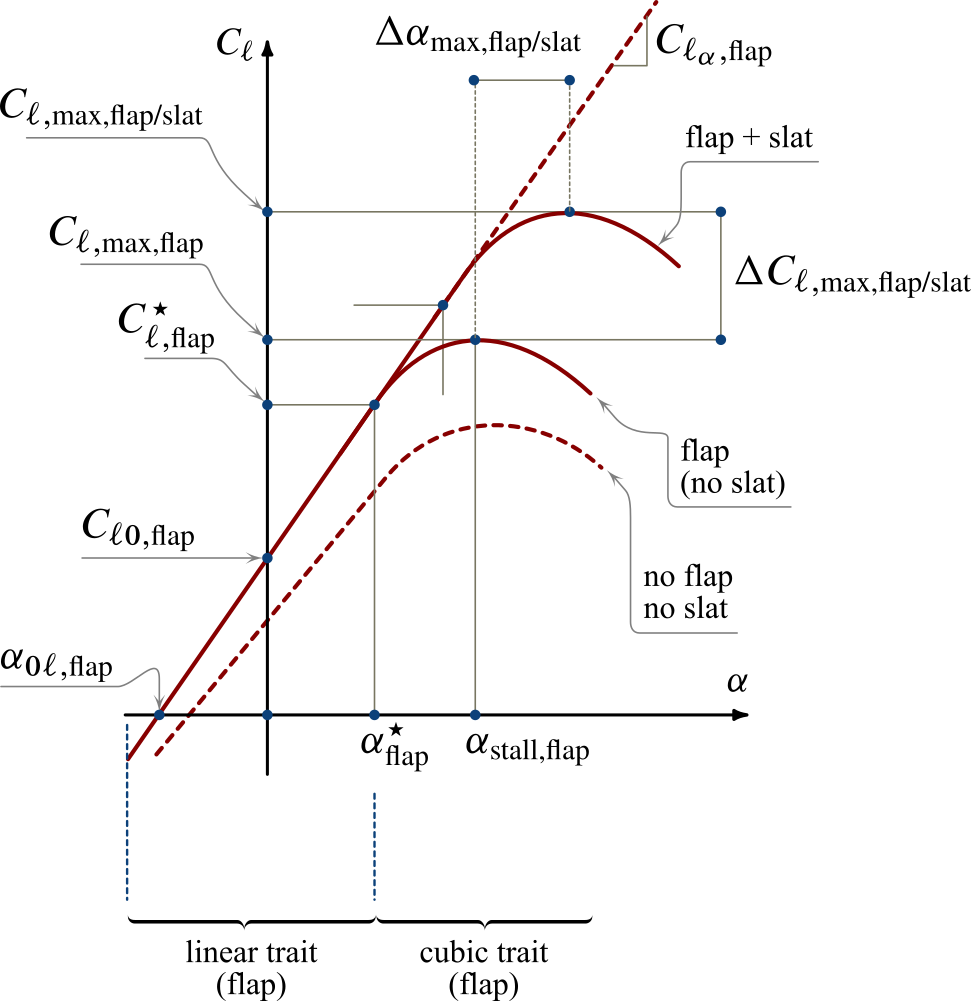
\includegraphics[width=\linewidth]{SlatEffects}
\captionof{figure}{Leading-edge devices effects}
\label{fig:SlatEffects}
\end{minipage}
\label{fig:FlapSlatEffects}
\end{figure}
%
\noindent
Among the variety of different devices, only the followings will be taken into account as they represents the most used ones.
%
\begin{itemize}
\item [\textbf{Plain flap}] This device is most used on small aircraft or ones equipped of a thin wing because it doesn't support a complex mechanism of retraction. Typical deflections are about 20° for take-off and 60° for landing.
\item [\textbf{Single slotted flap}]  It can be seen as a plain flap with a gap between the two elements composing the airfoil. The single slotted flap has very little flap overlap with the fixed trailing edge and hence develops only little Fowler motion, that is the aft travel of the flap that increases the section chord. Its typical deflections are about 20° for take-off and 45° for landing.
%
The effects of a single slotted flap show an increment in all the aerodynamic coefficients, but it must be said that the increment in drag is lower than that for plain flaps. The slotted flap chord usually ranges from the 25\% up to the 30\% of the section chord. Moreover the slot influences boundary layer control, in fact it introduces a blowing that energizes the boundary layer delaying separation, so an increase in lift is generated.
\item[\textbf{Double slotted flap}] This device is superior to the previous type at large deflections, because separation of the flow over the flap is postponed by the more favourable pressure distribution. Its typical deflections are about 20° for take-off and 50° for landing; in particular, in order to avoid an increasing twisting moment due the deflection, this devices are usually combined with leading edge slats deflected of the same quantity. 
\item[\textbf{Triple slotted flap}] This device is used on several transport aircraft with very high wing loadings. In combination with leading edge devices, this system represents almost the ultimate achievement in passive high-lift technology, but its shape shows that complicated flap supports and controls are required. Its typical deflections are about 20° for take-off and 50° for landing.
\item[\textbf{Fowler flap}]  It is theoretically a single slotted flap that adds to the downward deflection also a backward motion that allows the increment of the effective chord and camber.
%
Due to the necessity of keeping the rear part of the wing section extended out the main element its implementation system is usually more complicated than the single slotted flaps but its weight and costs are largely justified by its high lift effectiveness. Its typical deflection are about 40° for landing and 15° for take-off, smaller than other types because the chord extension provides a bigger lift increment due to the bigger wing surface; this also reduces the drag in take-off wth benefit an the required field length.
\item[\textbf{Slat}]  It's the most efficient leading edge device; thanks to combined deflection and forward motion, it acts in order to increase airfoil camber, and so the maximum lift coefficient, as well as increase the airfoil chord with the result of a bigger surface which provides a bigger aspect ratio with the effect of increase the lift curve slope of the linear trait. Furthermore, thanks to the slot which provides a boundary layer energization, it also increases the stalling angle of attack.
\item[\textbf{Krueger flap}]  It acts in the same way as the slat, but it is thinner and more suitable for installation on thin wings. Krueger flaps are very common because of their simple architecture.
\item[\textbf{Plain leading edge flap}] Is less effective than slat since it has no slot, it is mechanically simple and rigid and particularly suitable for thin airfoil sections. The leading edge can be hinged in order to move it backward (droop nose) or it has a mechanism inside that changes the curvature of the nose (variable camber flap).
\item[\textbf{Leading edge fixed slot}] It has a fixed slot at the leading edge that, at high angle of attack, allows the airflow to pass through energizing the boundary layer; this helps to increase the stalling angle of attack. During the cruise phase, in which the angle of attack is small, the gap is usually sealed.
\end{itemize}
%
\begin{figure}[!t]
  \centering
  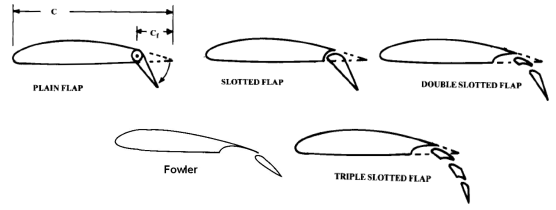
\includegraphics[width=\linewidth]{Flap}
  \caption{Analyzed trailing edge devices types}
  \label{fig:FlapTypes}
\end{figure}
%
\begin{figure}[!t]
  \centering
  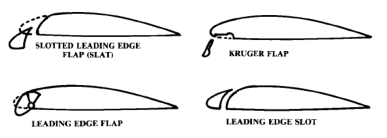
\includegraphics[width=0.7\linewidth]{Slat}
  \caption{Analyzed leading edge devices types}
  \label{fig:SlatTypes}
\end{figure}
%
\noindent
In order to predict, from the preliminary design phase, the aerodynamic characteristics of the high-lift devices, some useful semi-empirical methods are available; in this particular case the followings formulas and charts are taken from~\cite{torenbeek1982synthesis} and~\cite{sforza2014commercial}.

\bigskip
\noindent
The guideline that will be followed provides to analyze separately the trailing edge and the leading edge devices effects; moreover it will start by evaluating the changes in aerodynamic characteristics of airfoils for then extends these to entire wing.
%
From figures~\ref{fig:FlapEffects} and~\ref{fig:SlatEffects}, it's possible to understand that the main changes introduced by trailing edge, or leading edge, devices are related to the evaluation of four quantities:
%
\begin{itemize}
\item $\upDelta C_{l0}$
\item $\upDelta C_{l\text{max}}$
\item $C_{l\alpha, \text{flap}}$
\item $\upDelta\alpha_{\text{stall}}$
\end{itemize}
%
%------------------------- DeltaCl0 & DeltaCL0 subsection---------------------------
\subsection{$\upDelta C_{l0}$ and  $\upDelta C_{L0}$ calculation}
An empirical method for predicting airfoil lift increments at zero angle of attack for high-lift systems $\left(\upDelta C_{l0}\right)$ comes from the Glauert’s linearized theory for thin airfoils with flaps. A result obtained from this theory for the lift due to flap deflection is the following.
%
\begin{equation}
\alpha_\delta=1-\frac{\theta_f-\sin(\theta_f)}{\pi}
\label{eqn:AlphaDelta}
\end{equation}
%
\noindent
In particular $\theta_f$ can be calculated as follows.
%
\begin{equation}
\theta_f=\cos^{-1}\left(2\ \frac{c_f}{c}-1\right)
\label{eqn:ThetaF}
\end{equation}
%
\noindent
Known this value, it's possible to evaluate the theoretical $\Delta c_{l0}$ which can be calculated as proposed in (\ref{eqn:DeltaCl0}).
%
\begin{equation}
\upDelta C_{l0}=\alpha_\delta\ C_{l\alpha}\ \delta_f
\label{eqn:DeltaCl0}
\end{equation}
%
with $C_{l\alpha}$ equals to the linear slope of the llift curve of the airfoil, and $\delta_{f}$ the flap angular deflection. For large flap deflections and for the separation at large flap angles due to viscosity, linear theory is in error when compared with exact one, for this reason we assume the effectiveness factor $\eta_\delta$, so the formulation becomes the following.
%
\begin{equation}
\Delta C_{l0}'=\alpha_\delta\ C_{l\alpha}\ \delta_f\ \eta_\delta
\label{eqn:DeltaCl0EtaDelta}
\end{equation}
%
More in detail, $\eta_\delta$ can be evaluated from the charts provided in figures~\ref{fig:EtaDeltaPlain} and~\ref{fig:EtaDelta}.
%
\begin{figure}[!t]
  \centering
  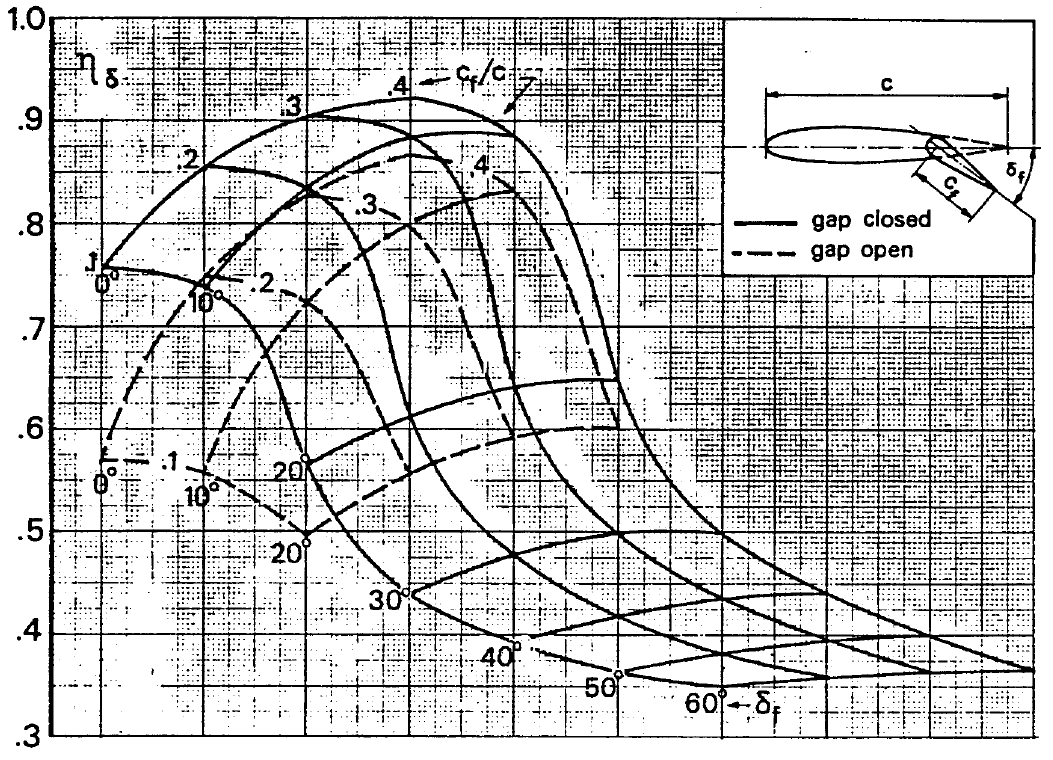
\includegraphics[width=0.7\linewidth]{Eta_Delta_Plain}
  \caption{$\eta_\delta$ for plain flap}
  \label{fig:EtaDeltaPlain}
\end{figure}
%
\begin{figure}[!b]
\centering
\makebox[\linewidth]{
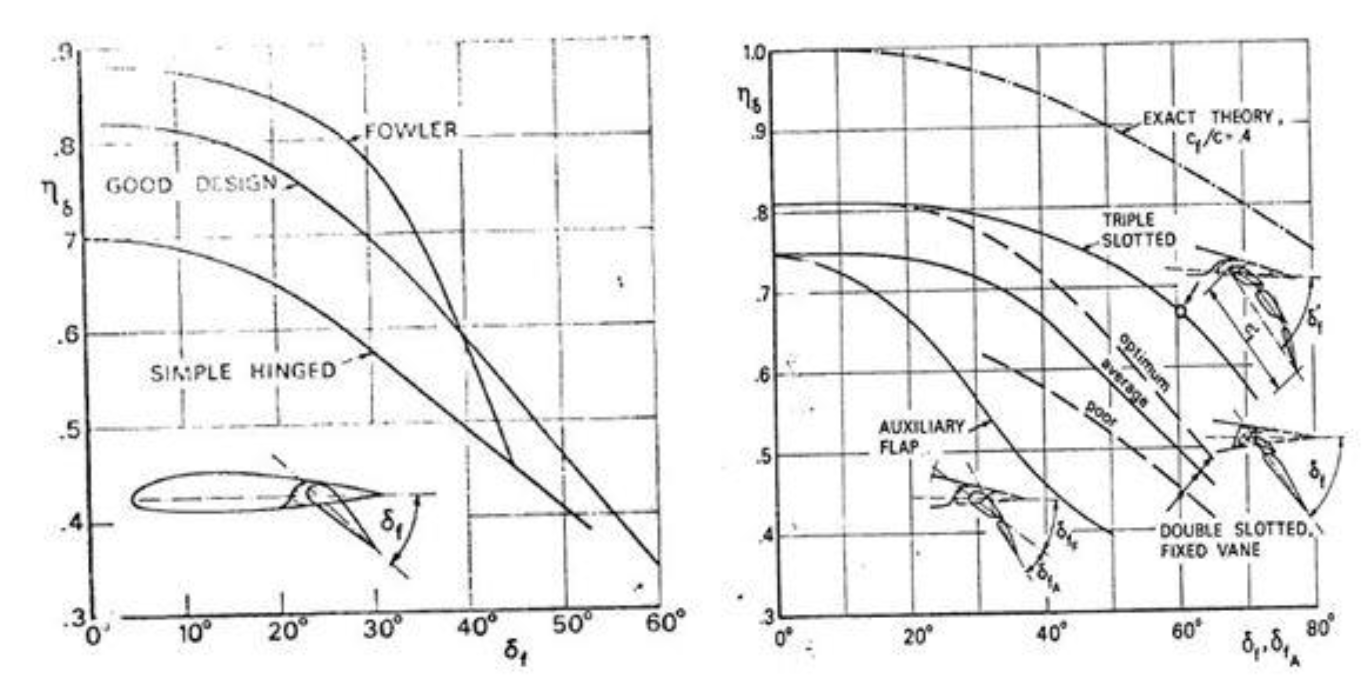
\includegraphics[width=1.1\linewidth, angle=359]{Eta_Delta}
}
\caption{$\eta_\delta$ for other type of flaps}
\label{fig:EtaDelta}
\end{figure}
%
\noindent
In case of flaps which extend the airfoil chord, this effects also contributes to the lift increase and can be taken into account by referring the section lift to the extended chord and then converting the result to the original chord. As a results of this, the section lift coefficient can be evaluated as shown in (\ref{eqn:clExtendedChord}).
%
\begin{equation}
C_{l}=\left(C_{l0}'+\upDelta C_{l0}'\right)\ \frac{c'}{c}
\label{eqn:clExtendedChord}
\end{equation}
%
\noindent 
Here the variables with superscript are referred to the extended chord. Assuming that for the basic section $C_{l0}'=C_{l0}$, it's possible to derive the $\upDelta C_{l0}$ as follows.
%
\begin{equation}
\upDelta C_{l0}=\upDelta C_{l0}'\ \frac{c'}{c}+C_{l0}\left(\frac{c'}{c}-1\right)
\label{eqn:Deltacl0Final}
\end{equation}
%
\noindent
In particular $C_{l0}$ is known, $\upDelta C_{l0}'$ is calculated as in (\ref{eqn:DeltaCl0EtaDelta}) and $\frac{c'}{c}$ is equal to the following~expression.
%
\begin{equation}
\frac{c'}{c}=1+\frac{\upDelta c}{c_f}\ \frac{c_f}{c}
\label{eqn:c'/c}
\end{equation}
%
\noindent
In particular $\frac{\upDelta c}{c_f}$ can be derived from the charts of figure~\ref{fig:DeltaCCf}.
%
\begin{figure}[!t]
  \centering
  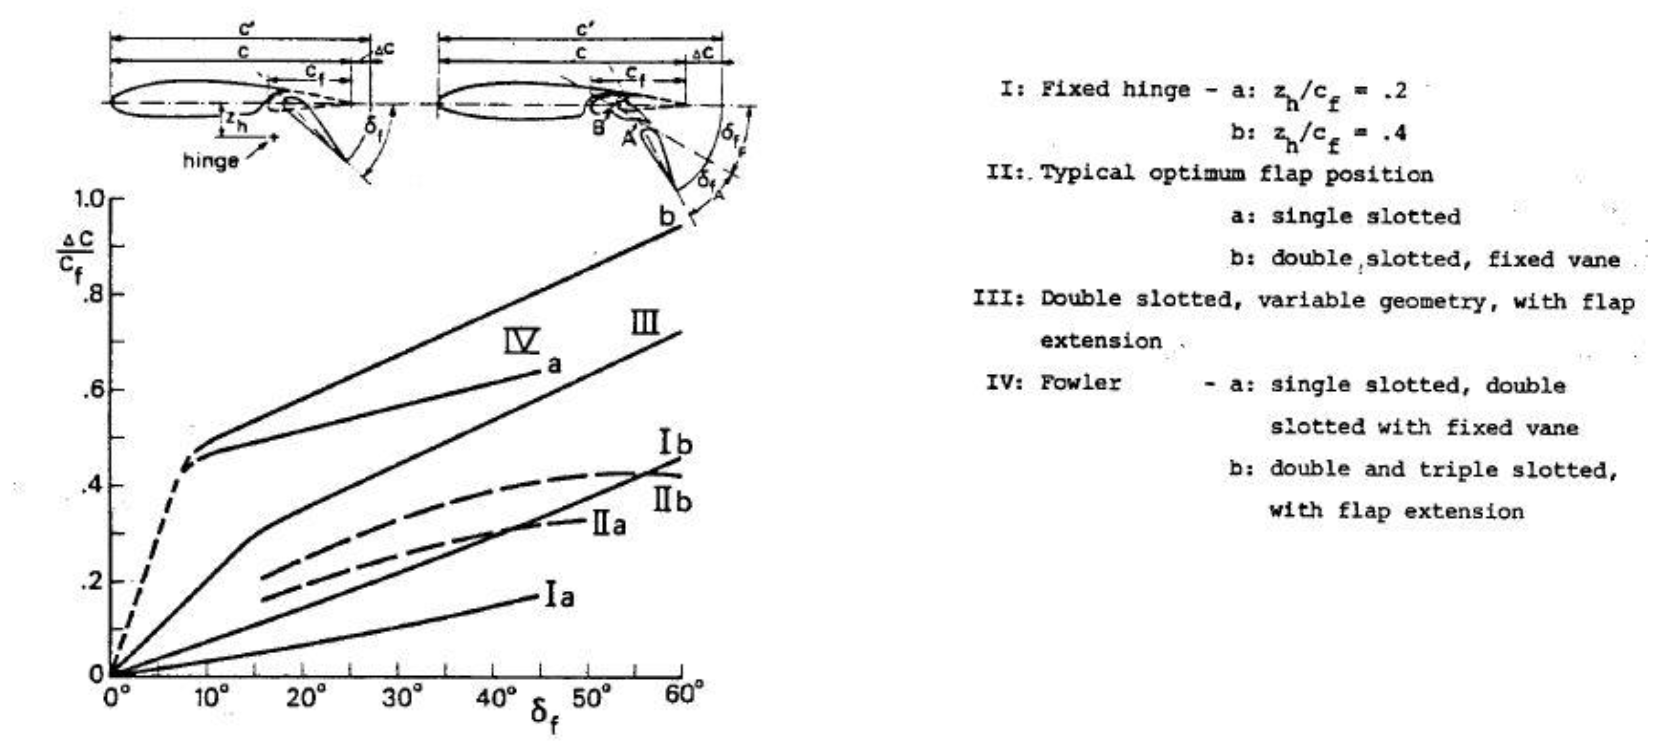
\includegraphics[width=\linewidth, angle=0.5]{DeltaC_Cf}
  \caption{$\frac{\upDelta c}{c_f}$ for different type of flaps as function of flap deflection}
  \label{fig:DeltaCCf}
\end{figure}
%
\noindent
The $\upDelta C_{l0}$ so calculated has now to be extended to the entire wing; this can be through the following formula.
%
\begin{equation}
\upDelta C_{L0}=\upDelta C_{l0}\ \left(\frac{C_{L\alpha}}{C_{l\alpha}}\right)\ \left[\frac{\left(\alpha_\delta\right)_{C_{L}}}{\left(\alpha_\delta\right)_{C_{l}}}\right]\ K_b
\label{eqn:c'/c}
\end{equation}
%
\noindent
where $C_{L\alpha}$ and $C_{l\alpha}$ are respectively the lift curve slopes of the wing and the airfoil, $\left[\left(\alpha_\delta\right)_{C_{L}}/\left(\alpha_\delta\right)_{C_{l}}\right]=K_c$ is the ratio of the three-dimensional flap effectiveness parameter to the two dimensional flap effectiveness one, which can be derived from the figure~\ref{fig:Kc}, and $K_b$ is a flap span effectiveness factor, which is function of the flap span-wise extension, that can be  read from~\ref{fig:Kb}.
%
\begin{figure}[!b]
  \centering
  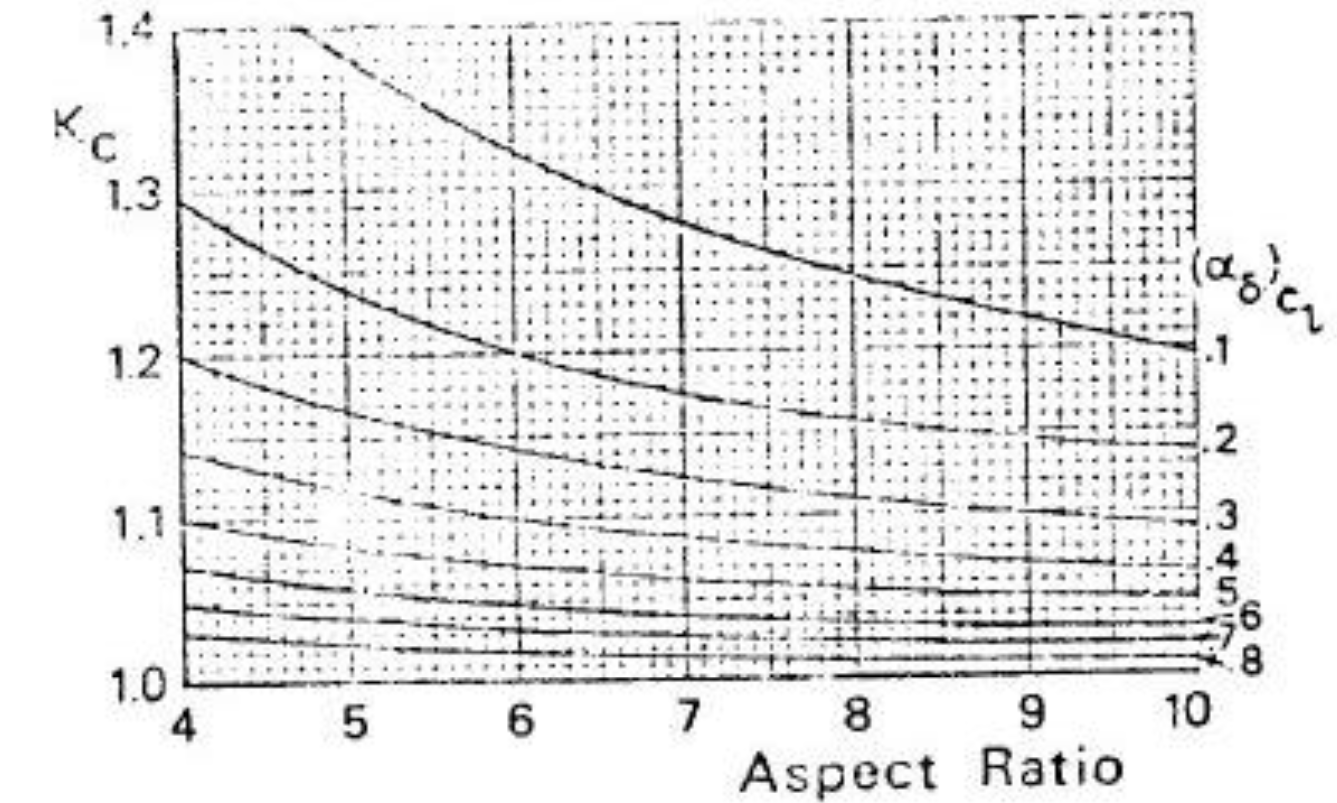
\includegraphics[width=0.7\linewidth, angle=359]{Kc}
  \caption{$K_c$ for different $\left(\alpha_\delta\right)_{C_{L}}$ as function of wing aspect ratio}
  \label{fig:Kc}
\end{figure}
%
\begin{figure}[!t]
  \centering
  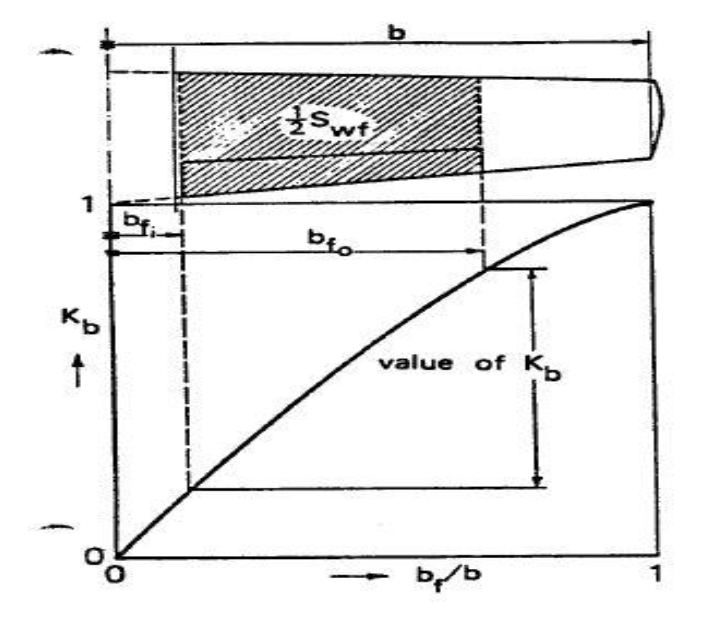
\includegraphics[width=0.55\linewidth]{Kb}
  \caption{$K_b$ as function of flap span to wing span ratio ($\frac{b_f}{b}$)}
  \label{fig:Kb}
\end{figure}
%
%------------------------- DeltaClmax & DeltaCLmax subsection---------------------------
\subsection{$\upDelta C_{l\text{max}}$ and  $\upDelta C_{L\text{max}}$ calculation for trailing edge and leading edge devices}
An empirical method for predicting airfoil maximum lift increments for plain and slotted flaps is presented in \gls{DATCOM} and will be followed from~\cite{sforza2014commercial}.
%
The maximum lift increment provided to an airfoil by the deflection of a trailing edge flap is given by the (\ref{eqn:DeltaClmaxFlap}).
%
\begin{equation}
\upDelta C_{l\text{max}}=k_1\ k_2\ k_3\ \left(\upDelta C_{l\text{max}}\right)_{\text{base}}
\label{eqn:DeltaClmaxFlap}
\end{equation}
%
\noindent
Here $\left(\upDelta C_{l\text{max}}\right)_{\text{base}}$ is the section maximum lift increment for 25 percent-chord flaps at the reference flap-deflection angle and is shown in figure~\ref{fig:DeltaClmaxBase} for different flap systems. The quantity $k_1$ is a factor accounting for flap-chord-to-airfoil-chord ratios, $\frac{c_{f}}{c}$, other than 0.25 and is shown in figure~\ref{fig:k1}. The quantity $k_2$ is a factor accounting for flap deflections other than the reference value and is shown in figure~\ref{fig:k2}. Finally, $k_3$ is a factor accounting for flap motion as a function of flap deflection and is shown in figure~\ref{fig:k3}.
%
\begin{figure}[!b]
  \centering
  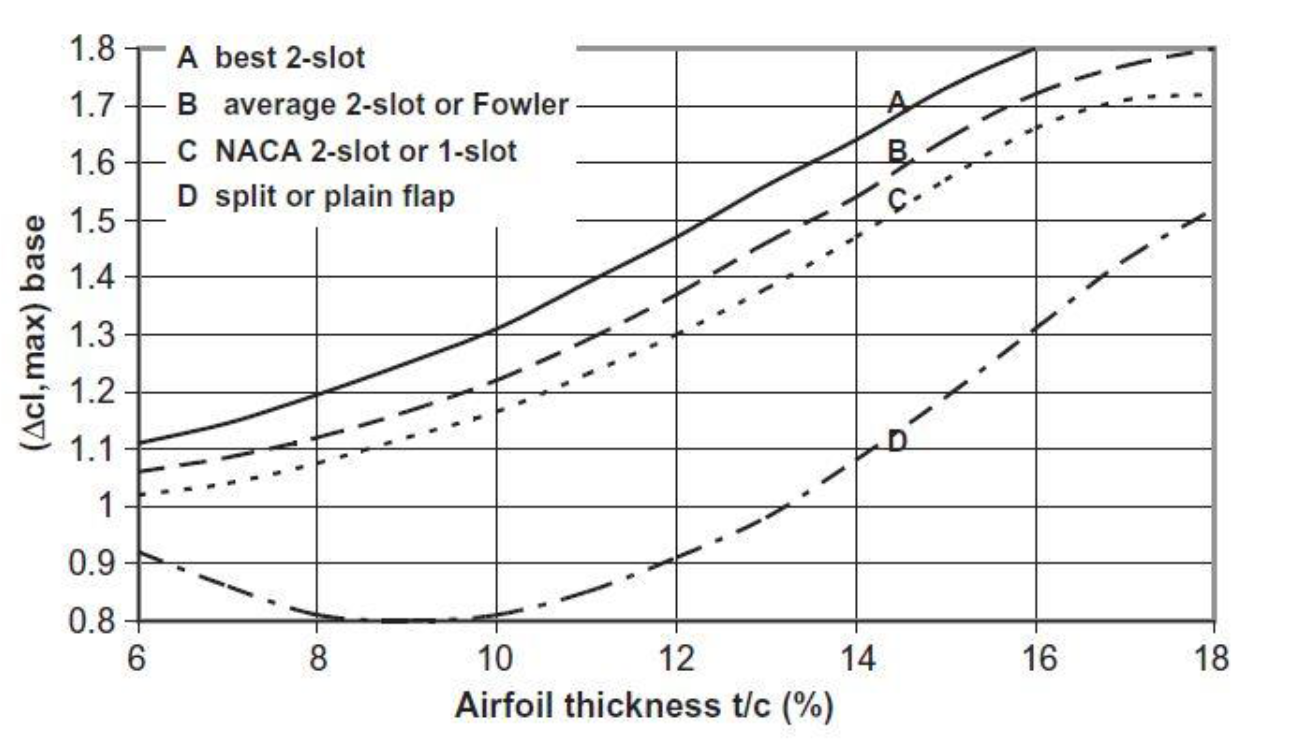
\includegraphics[width=0.67\linewidth]{DeltaClmax_Base}
  \caption{$\left(\upDelta C_{l\text{max}}\right)_{\text{base}}$ DATCOM chart}
  \label{fig:DeltaClmaxBase}
\end{figure}
%
\begin{figure}[H]
  \centering
  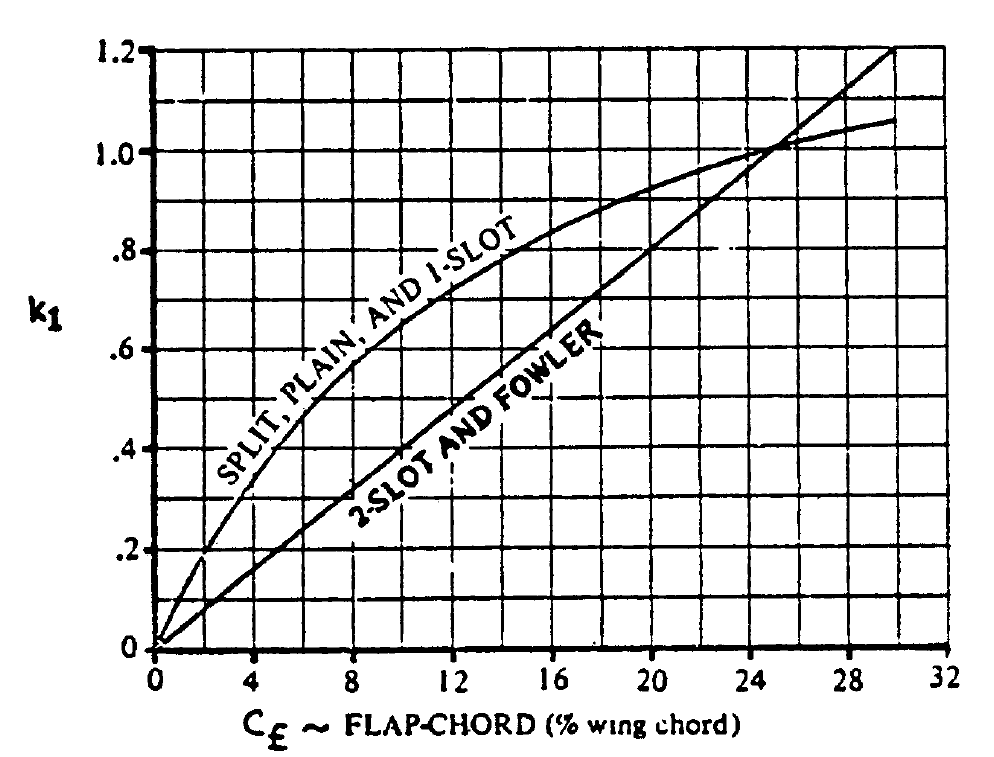
\includegraphics[width=0.8\linewidth]{K1}
  \caption{$k_1$ correction factor for trailing edge flap chord to airfoil-chord ratios, $\frac{c_{f}}{c}$, other than 0.25}
  \label{fig:k1}
\end{figure}
%
\begin{figure}[H]
\centering
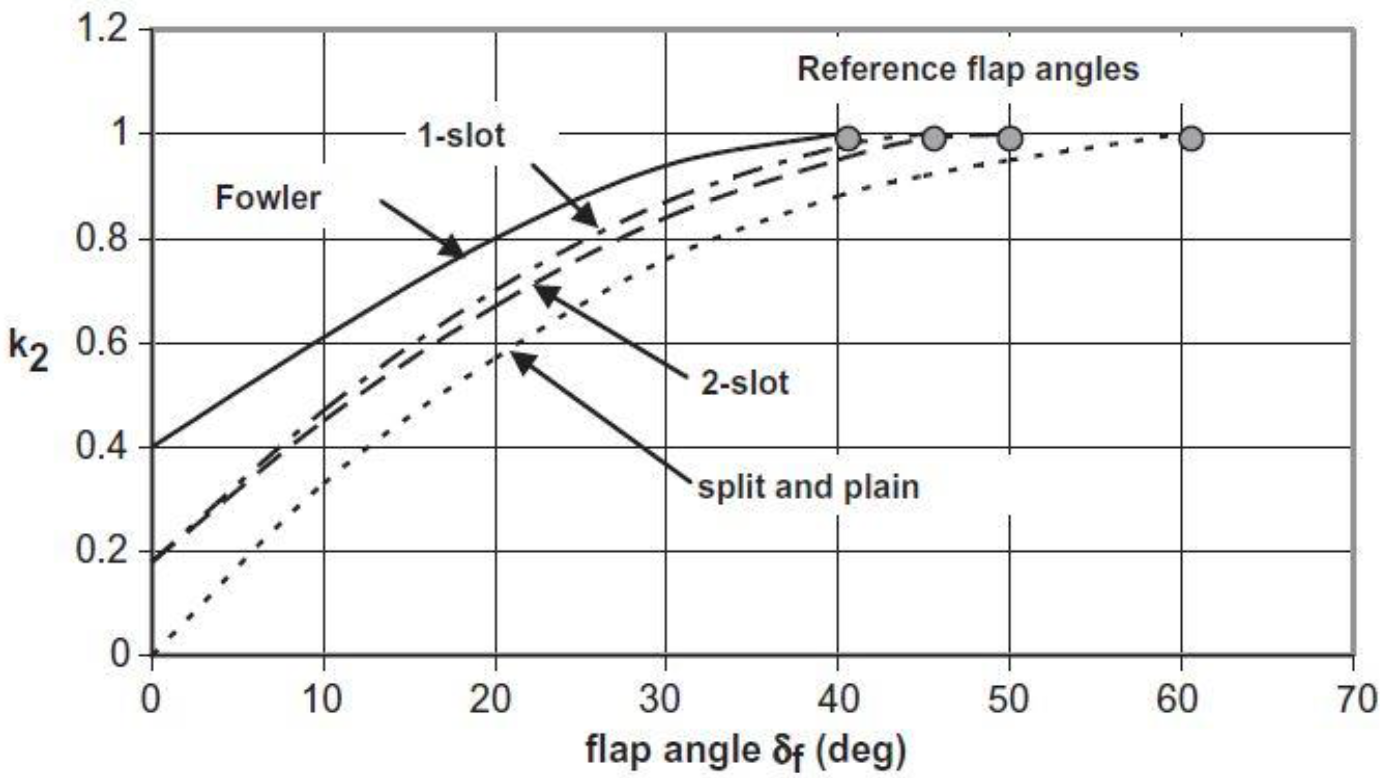
\includegraphics[width=0.8\linewidth]{K2}
\caption{Flap angle correction factor $k_2$. The reference flap angle for each type of flap is shown as a solid symbol at $k_2=1$}
\label{fig:k2}
\end{figure}
%
\begin{figure}[H]
\centering
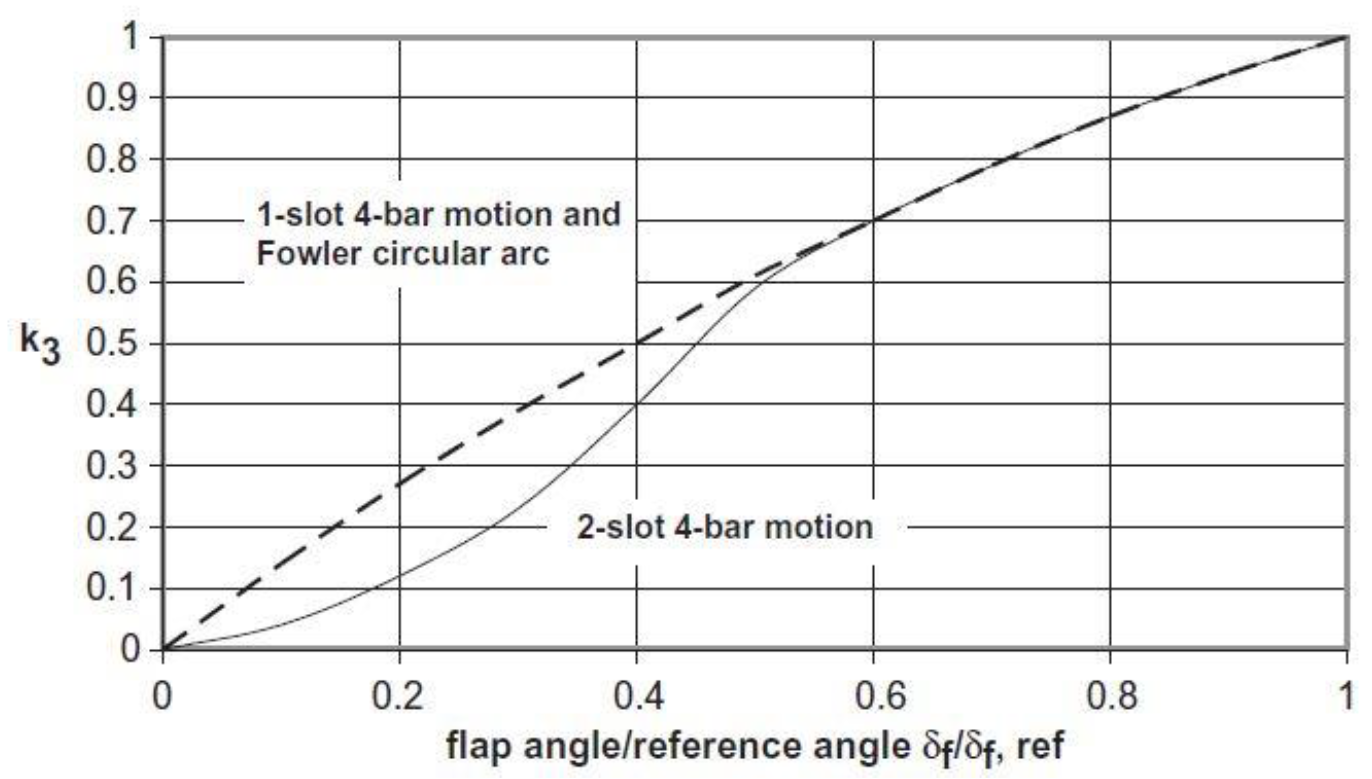
\includegraphics[width=0.8\linewidth]{K3}
\caption{Flap motion correction factor $k_3$}
\label{fig:k3}
\end{figure}
%
\noindent
Regarding leading edge devices, the leading edge slats are the most common ones; as explained previously, the latter increase the maximum lift coefficient of the airfoil along with the stall angle. As a result, they are commonly used, particularly in landing, though they are also useful on takeoff because the lift increment they develop comes with little drag penalty.
%
The \gls{DATCOM} method for leading edge flaps and slats proposes that the maximum lift increment for leading edge flaps or slats may be approximated by the following empirical relation.
%
\begin{equation}
\upDelta C_{l\text{max}}=\left(\dfrac{\partial C_l}{\partial \delta}\right)_{\text{max}}\ \eta_{\text{max}}\ \eta_\delta\ \delta_s\ \dfrac{c'}{c}
\label{eqn:DeltaClmaxSlat}
\end{equation}
%
\noindent
The first term in the previous equation is the theoretical lift effectiveness which gives the rate of change of the lift coefficient with change in deflection angle; it is shown in figure~\ref{fig:dCldDelta} as a function of the leading edge flap, or slat, chord to airfoil-chord ratio $\frac{c_s}{c}$.
%
The second term, $\eta_{\text{max}}$, is an empirical factor which accounts for the effects of airfoil leading edge radius and maximum thickness. A graph of this factor is presented in figure~\ref{fig:etaDeltaMaxSlat}; the discontinuity in the curve for slats is said to be due to a lack of data in the region of the discontinuity, but an \emph{ad hoc} correction is also proposed in order to provide more accurate results.
%
The third term, $\eta_\delta$, is another empirical factor which corrects for flap, or slat, deflections different from the optimum flap angle. This parameter is shown in figure~\ref{fig:etaDeltaSlat} as a function of the flap, or slat, deflection angle $\delta_s$. To understand the angle $\delta_s$ one may first imagine
drawing a chord line on the slat-airfoil combination when the slat is stowed; then when the slat is deflected, the segment of the chord line that was drawn on
the slat in the stowed position has now rotated through the deflection angle $\delta_s$. This is the standard used in the \gls{DATCOM} method and is not necessarily used throughout the literature as a definition of slat deflection angle.
%
Finally, the ratio $\frac{c'}{c}$ accounts for the apparent increase in chord length when the slat is deflected and a slot is formed between the two airfoil elements; this dimension, along with the deflection angle $\delta_s$, is illustrated in figure~\ref{fig:c'c_deltaSlat}.
%
\begin{figure}[H]
\centering
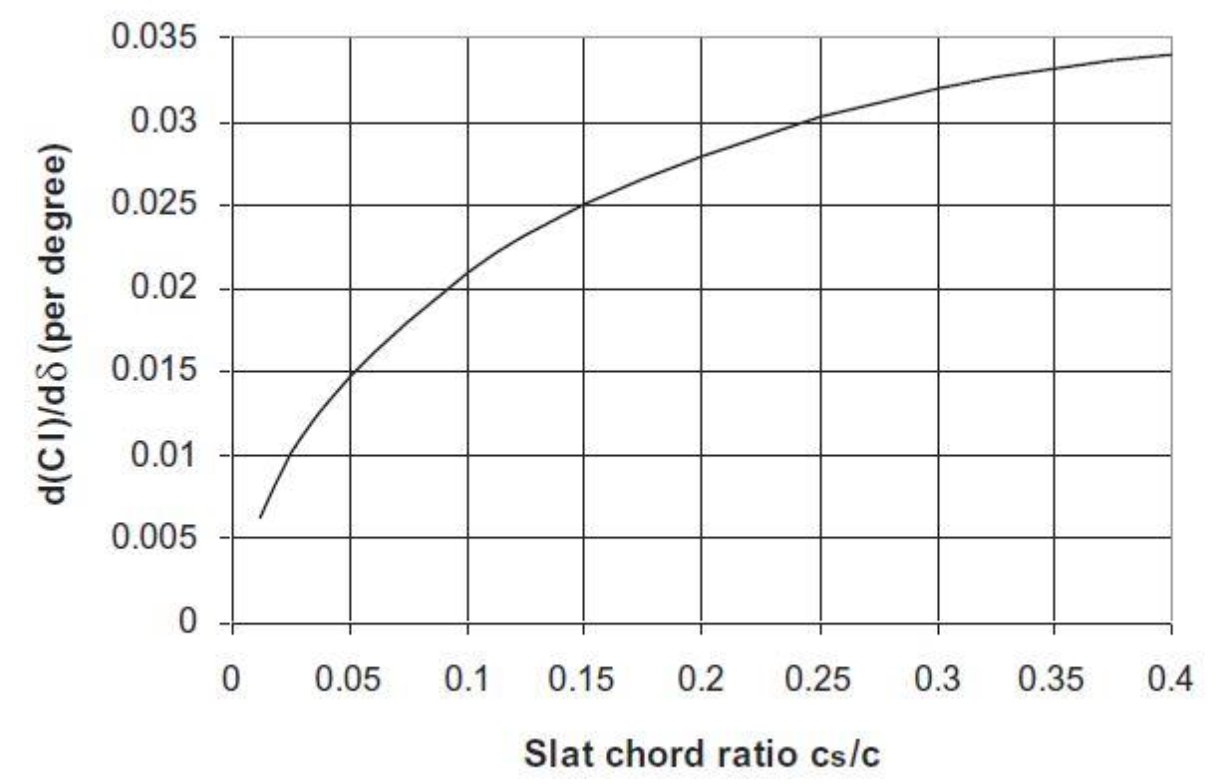
\includegraphics[width=0.8\linewidth]{DeltaCl_Ddelta}
\caption{Rate of change of airfoil lift coefficient with slat deflection (per degree)}
\label{fig:dCldDelta}
\end{figure}
%
\begin{figure}[H]
\centering
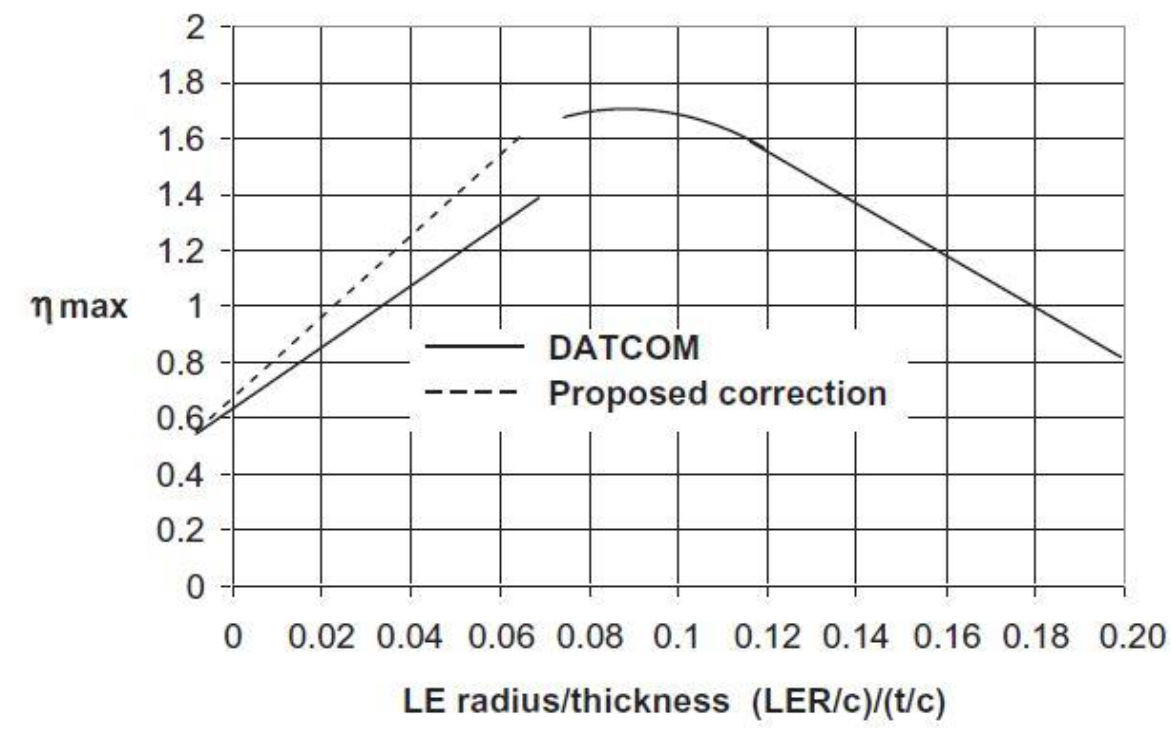
\includegraphics[width=0.8\linewidth]{Eta_max}
\caption{Correction factor for leading edge radius and airfoil thickness ratio}
\label{fig:etaDeltaMaxSlat}
\end{figure}
%
\begin{figure}[H]
\centering
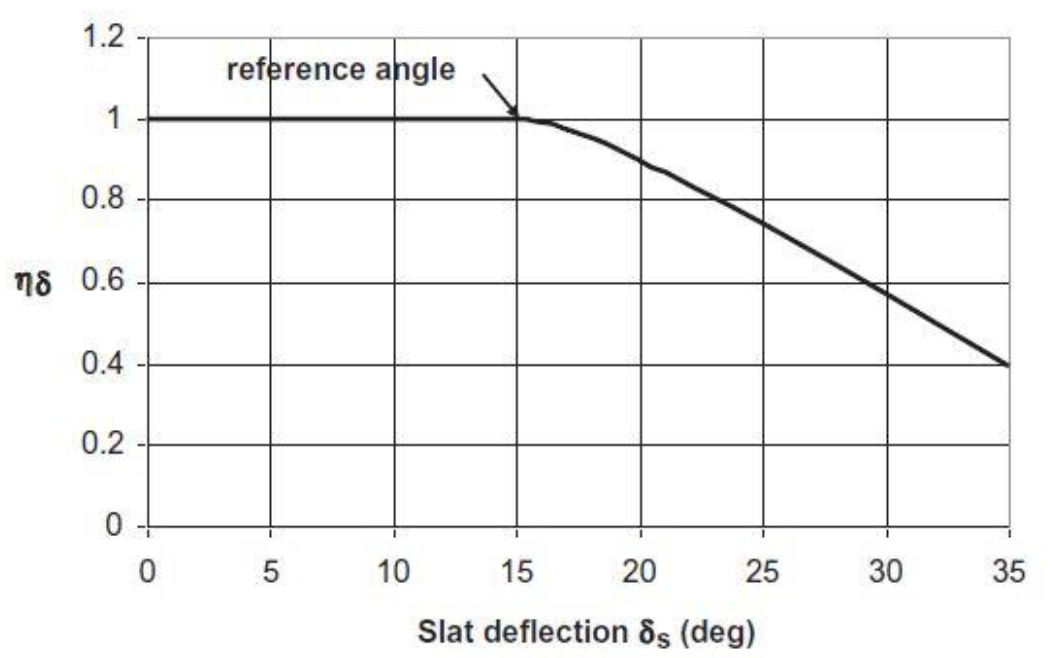
\includegraphics[width=0.8\linewidth]{Eta_Delta_Slat}
\caption{Slat deflection correction factor as a function of deflection angle}
\label{fig:etaDeltaSlat}
\end{figure}
%
\begin{figure}[H]
\centering
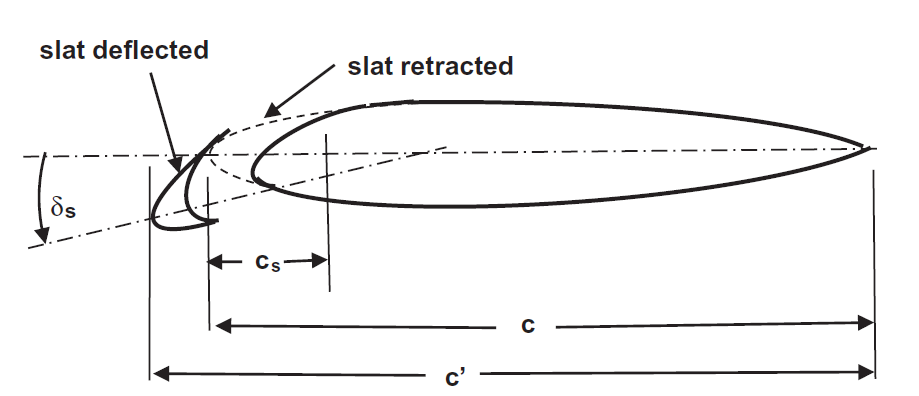
\includegraphics[width=0.8\linewidth]{deltaSlat_c'c}
\caption{Geometry of the leading edge as used in the \gls{DATCOM} method}
\label{fig:c'c_deltaSlat}
\end{figure}
%
\noindent
Now that all increments related to the airfoil have been explained, the next step is to extend these two-dimensional quantities to the entire three-dimensional wing.
Regarding trailing edge devices, the \gls{DATCOM} method provides the following equation to compute the increment in maximum lift coefficient for the wing.
%
\begin{equation}
\upDelta C_{L\text{max}}=\upDelta C_{l\text{max}}\ \dfrac{S_{w,f}}{S}\ K_\Lambda
\label{eqn:DeltaCLmaxFlap}
\end{equation}
%
\noindent
Here $\upDelta C_{l\text{max}}$ is the increment in lift coefficient due to flap deflection as defined in (\ref{eqn:DeltaClmaxFlap}) while the quantity $\frac{S_{w,f}}{S}$ is the ratio of wing area affected by the trailing edge flap deflection (including both port and starboard wings) to the total wing area, as shown in figure~\ref{fig:Swf}; the wing area affected by the flap may be written as in (\ref{eqn:Swf}).
%
\begin{equation}
S_{w,f}=\left(\dfrac{b}{2}\right)c_r\left[2-\left(1-\lambda\right)\left(\eta_{\text{in}}-\eta_{\text{out}}\right)\right]\left(\eta_{\text{in}}-\eta_{\text{out}}\right)
\label{eqn:Swf}
\end{equation}
%
\begin{figure}[!b]
\centering
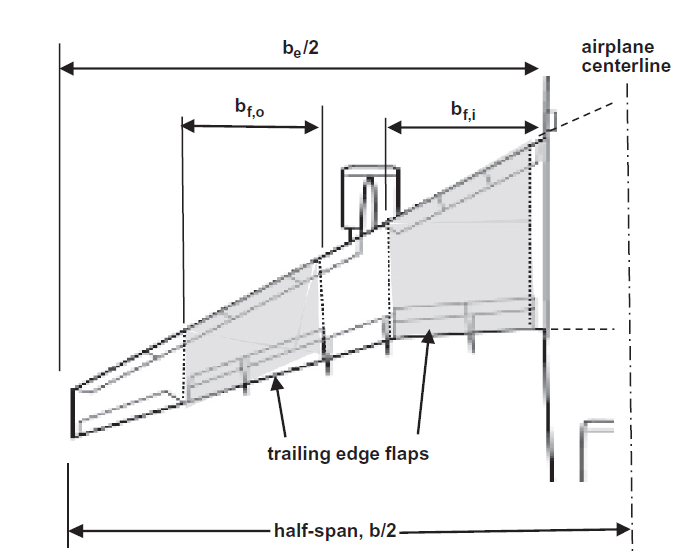
\includegraphics[width=0.75\linewidth]{Swf}
\caption{Plan view of wing where shaded area, including both the starboard and port wing, is the rated area for the flaps, that is, the portion of the wing planform area affected by the flaps}
\label{fig:Swf}
\end{figure}
%
\noindent
In the (\ref{eqn:Swf}) the quantity $\lambda=\frac{c_t}{c_r}$ is the taper ratio and b is the wingspan; while $\eta_i$ and $\eta_o$ are, respectively, the non-dimensional inboard location and the outboard location of the flap. If the flaps do not extend continuously along the trailing edge then the affected area for each may be calculated independently and added together.

\bigskip
\noindent
Finally the correction factor for sweepback wings is given by the following equation.
%
\begin{equation}
K_\Lambda=\left(1-0.08\ \cos^2\Lambda_{c/4}\right)\ \cos^{3/4}\Lambda_{c/4}
\label{eqn:KLambda}
\end{equation}
%
\noindent
The same calculations provided for trailing edge devices can be used for leading edge devices as well with the difference that the $\upDelta C_{l\text{max}}$ has to be calculated with the (\ref{eqn:DeltaClmaxSlat}). 
%
%--------------------------- Cl_alpha & CL_alpha subsection-------------------------------
\subsection{$C_{l\alpha, \text{flap}}$ and  $C_{L\alpha, \text{flap}}$ calculation}
The lift gradient is affected by flap deflection in three ways:
%
\begin{itemize}
\item The chord extension increases $C_{l\alpha}$. This effect depends on the multiplicative factor $\frac{c'}{c}$
\item The potential flow effect of flap deflection on the lift curve slope is reduced with increasing $\alpha$. The result is a nonlinearity in the lift curve which is particularly pronounced for large flap angles.
\item The effect of viscosity on the lift effectiveness of a flap increases with the angle of attack, thus reducing $\left(\upDelta C_{l}\right)_{\text{flap}}$ with increasing $\alpha$
\end{itemize}
%
\noindent
In order to evaluate the variation in $C_{l\alpha}$ due to flap deflection, references to~\cite{torenbeek1982synthesis} have been made. In particular, Torenbeek provides the following equation which approximates the results of the exact theory fairly accurately and is in qualitative agreement with experimental data. 
%
\begin{equation}
C_{l\alpha_{\left(\text{flap down}\right)}}=C_{l\alpha}\ \left[\dfrac{c'}{c}\ \left(1-\dfrac{c_f}{c'}\ \sin^2\delta_f\right)\right]
\label{eqn:ClalphaFlap}
\end{equation}
%
\noindent
This equation is then corrected for the three-dimensional wing as follows.
%
\begin{equation}
C_{L\alpha_{\left(\text{flap down}\right)}}=C_{L\alpha}\ \left\{1+\dfrac{\upDelta C_{L0}}{\upDelta C_{l0}}\ \left[\left(\dfrac{c'}{c}\ \left(1-\dfrac{c_f}{c'}\sin^2\delta_f\right)-1\right)\right]\right\}
\label{eqn:ClalphaFlap}
\end{equation}
%
%------------------------------ DeltaAlphaMax subsection-----------------------------------
\subsection{$\upDelta\alpha_{\text{stall}}$ calculation for trailing edge and leading edge devices}
As explained previously, trailing edge devices contribute to lower the stalling angle of attack, while leading edge devices do the opposite providing an higher $\alpha_{\text{stall}}$. 
%
In order to compute these two effects, a reference to~\cite{nicolai2010fundamentals} has been done; in particular, the value of $\upDelta\alpha_{\text{stall}}$ is taken as the same used in the construction of the clean wing lift curve; the latter shown in figure~\ref{fig:DeltaAlphaMaxFlap}.
%
\begin{figure}[H]
\centering
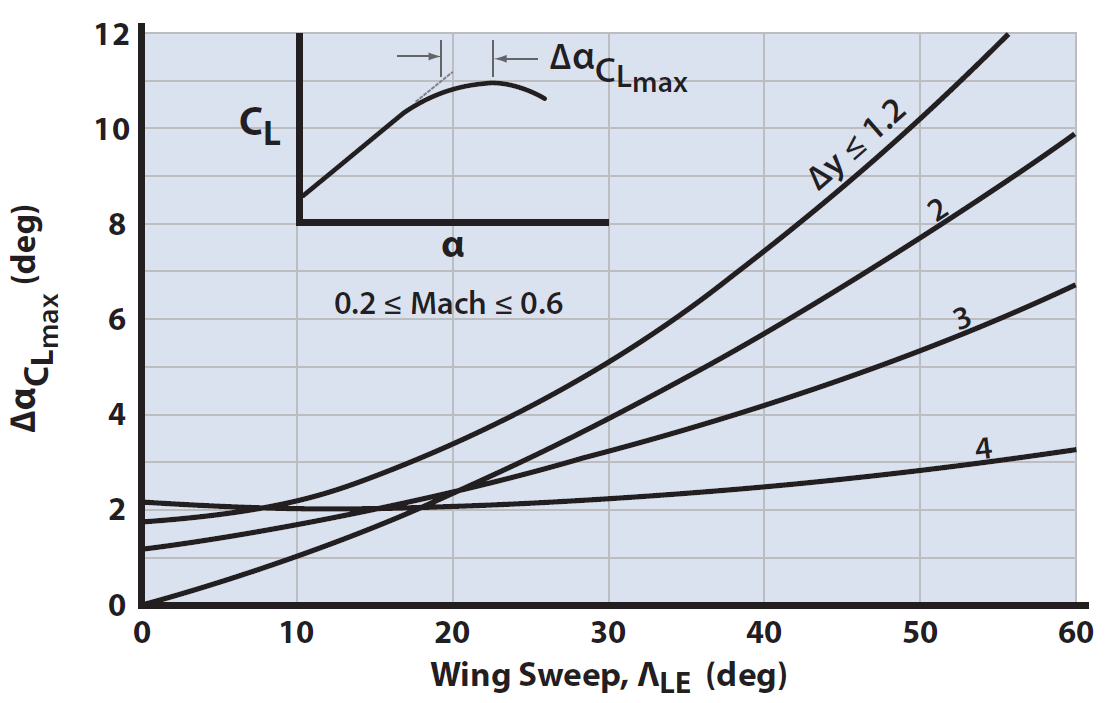
\includegraphics[width=0.8\linewidth]{DeltaAlphaMaxFlap}
\caption{$\upDelta\alpha_{\text{stall}}$ as function of the sweep angle and of the leading edge sharpness parameter $\frac{\upDelta y}{c}$}
\label{fig:DeltaAlphaMaxFlap}
\end{figure}
%
\noindent
where the airfoil leading edge sharpness parameter, $\frac{\upDelta y}{c}$, can be estimated from the following chart.
%
\begin{figure}[H]
\centering
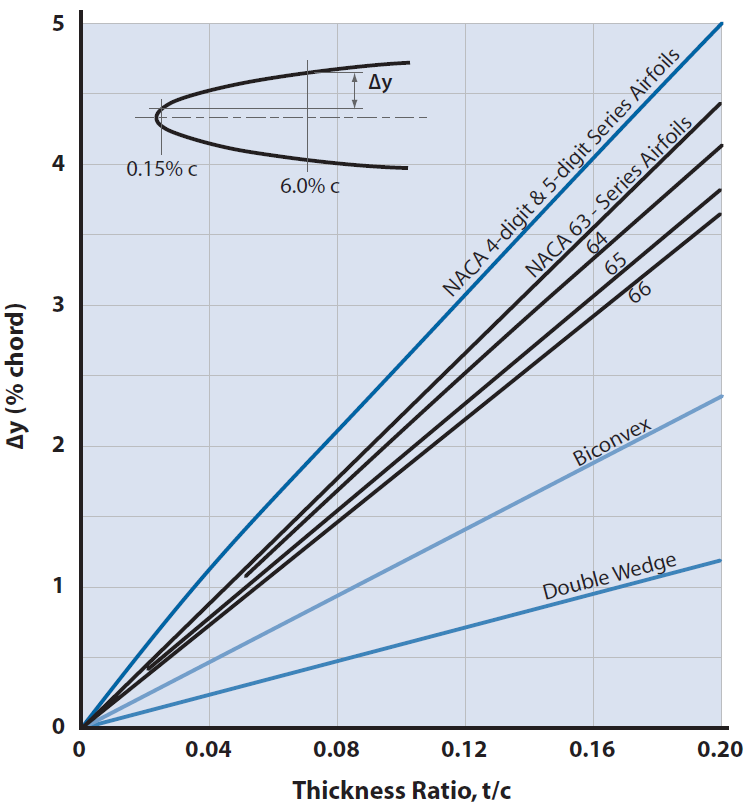
\includegraphics[width=0.8\linewidth]{DeltaY}
\caption{Variation of LE sharpness parameter with airfoil thickness ratio}
\label{fig:DeltaY}
\end{figure}
%
%---------------------------  DeltaCD0 & DeltaCM subsection--------------------------------
\subsection{Further effects calculations}\label{subpar:DCD0}
High-lift devices influence not only the lift curve but also the wing drag polar, in particular the $C_{D0}$, and the wing pitching moment. Further calculations are, therefore, necessary to predict these latter. Regarding the $\upDelta C_{D0}$ provided by high-lift devices, the reader can refer to~\cite{Young:Flaps}. Proceeding on much the same lines as in the analysis of lift coefficient increments, Young and Hufton assumed that  $\upDelta C_D0$ can be calculated as follow for a full-span flap.
%
\begin{equation}
\upDelta C_{D0}=\delta_1\left(c_f/c\right)\cdot\delta_2\left(\delta_f\right)
\label{eqn:DeltaCD0FullSpan}
\end{equation}
%
where $\delta_1$ and $\delta_2$ are functions that were determined from experimental data. Their related curves are shown in figure~\ref{fig:Delta1Plain} and~\ref{fig:Delta2Plain}, for plain flap, and, in figure~\ref{fig:Delta1Slotted} and~\ref{fig:Delta2Slotted}, for slotted flaps.
%
\begin{figure}[H]
\centering
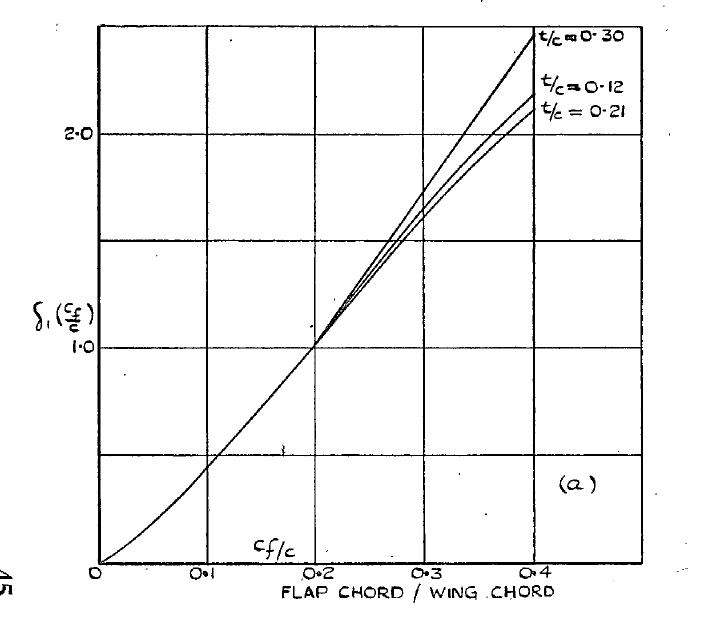
\includegraphics[width=0.9\linewidth]{Delta1_Plain}
\caption{The functions $\delta_1\left(c_f/c\right)$ for split and plain flaps}
\label{fig:Delta1Plain}
\end{figure}
%
\begin{figure}[H]
\centering
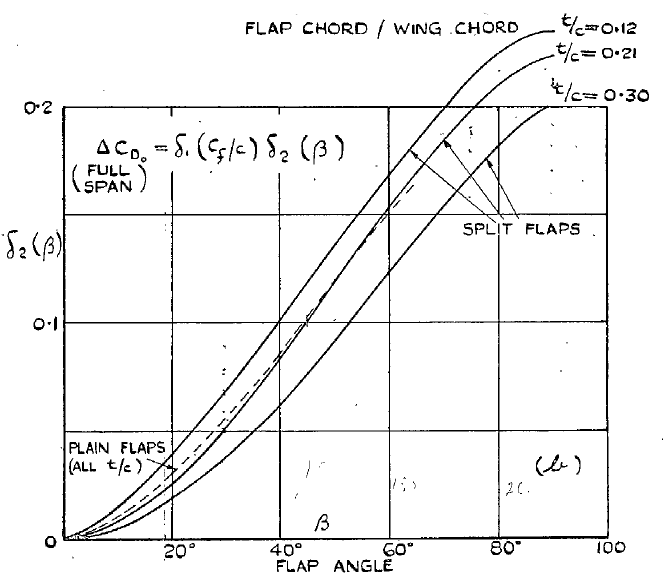
\includegraphics[width=0.7\linewidth]{Delta2_Plain}
\caption{The functions $\delta_2\left(\delta_f\right)$ for plain flaps}
\label{fig:Delta1Slotted}
\end{figure}
%
\begin{figure}[H]
\centering
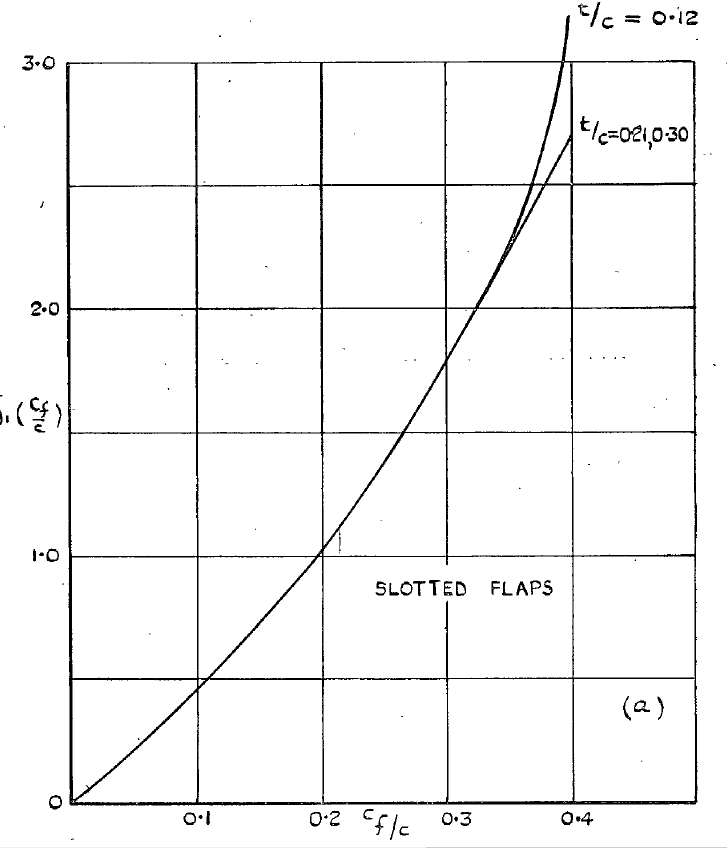
\includegraphics[width=0.7\linewidth]{Delta1_Slotted}
\caption{The functions $\delta_1\left(c_f/c\right)$ for split and slotted flaps}
\label{fig:Delta2Plain}
\end{figure}
%
\begin{figure}[H]
\centering
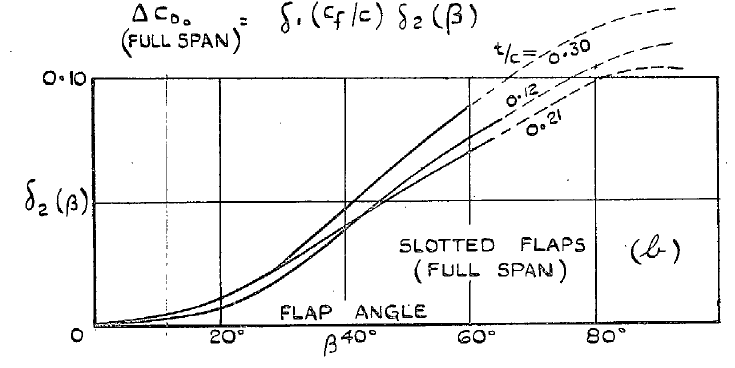
\includegraphics[width=0.7\linewidth]{Delta2_Slotted}
\caption{The functions $\delta_2\left(\delta_f\right)$ for slotted flaps}
\label{fig:Delta2Slotted}
\end{figure}

\bigskip
\noindent
General considerations, confirmed by experimental data, led Young and Hufton to conclude that the drag increment of a part-span flap of any type is proportional to the area of the flapped part of the wing.
%
\noindent
Hence, to determine the increment for a part-span flap it's necessary to multiply the increment for a full-span flap by the ratio of the flapped wing area to the total wing area. The latter ratio, denoted by $\delta_3$, is shown in figure~\ref{fig:Delta3} as a function of flap span for wings of various taper~ratios. Thus the $\upDelta C_{D0}$ equation becomes the following.
%
\begin{equation}
\upDelta C_{D0}=\delta_1\left(c_f/c\right)\cdot\delta_2\left(\delta_f\right)\cdot\delta_3\left(b_f/b\right)
\label{eqn:DeltaCD0PartSpan}
\end{equation}
%
\begin{figure}[!t]
\centering
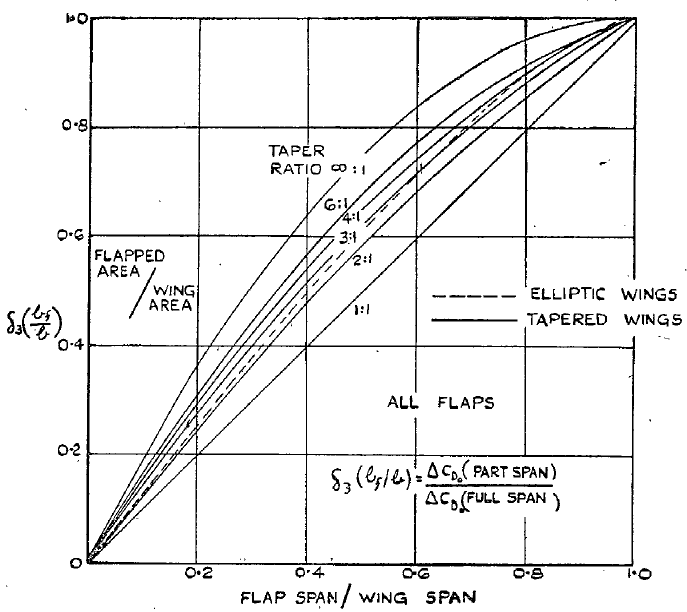
\includegraphics[width=0.7\linewidth]{Delta3}
\caption{The functions $\delta_3\left(b_f/b\right)$ for slotted flaps}
\label{fig:Delta3}
\end{figure}
%
The last, but not least, effect to be predict refers to the pitching moment of the airfoil and of the wing. Following the guideline proposed in~\cite{torenbeek1982synthesis}, the generalized expression, for airfoils, in (\ref{eqn:DeltaCm}) represents a useful starting point when experimental data are not available.
%
\begin{equation}
\upDelta C_{m_{\frac{c}{4}}}=-\mu_1\ \upDelta C_{l\text{max}}\ \left(\dfrac{c'}{c}\right)^2-\dfrac{C_l}{4}\ \dfrac{c'}{c}\left(\dfrac{c'}{c}-1\right)+\left(C_{m_{\frac{c}{4}}}\right)_{\delta_f=0}\ \left[\left(\dfrac{c'}{c}\right)^2-1\right]
\label{eqn:DeltaCm}
\end{equation}
%
where extended chord $c'$, shown in figure~\ref{fig:DeltaCCf}, allows for the effects of the backward movement of the flap while it is being extended.
%
In equation this equation, the first contribution is due to the increased section camber and the factor $\mu_1$ is defined as follows according to Glauert's linear theory for small flap deflections.
%
\begin{equation}
\mu_1=\dfrac{1}{2}\left(1-\dfrac{c_f}{c}\right)\dfrac{\sin\theta_f}{\pi-\left(\theta_f-\sin\theta_f\right)}
\label{eqn:Mu1}
\end{equation}
%
where $\theta_f$ is the one from equation (\ref{eqn:ThetaF}). This theoretical value of $\mu_1$ generally underestimate the pitching moment coefficient; in fact it has been found that, for slotted flaps with, or without, Fowler movement, most data are on a single line, provided the second term of the equation (\ref{eqn:Mu1}), representing the theoretical rearward shift of the airfoil aerodynamic center, is halved. Furthermore, in the case of split and plain flaps, the flap angle is observed to exert a pronounced influence on $\mu_1$ as shown in figure~\ref{fig:Mu1}.
%
\begin{figure}[!t]
\centering
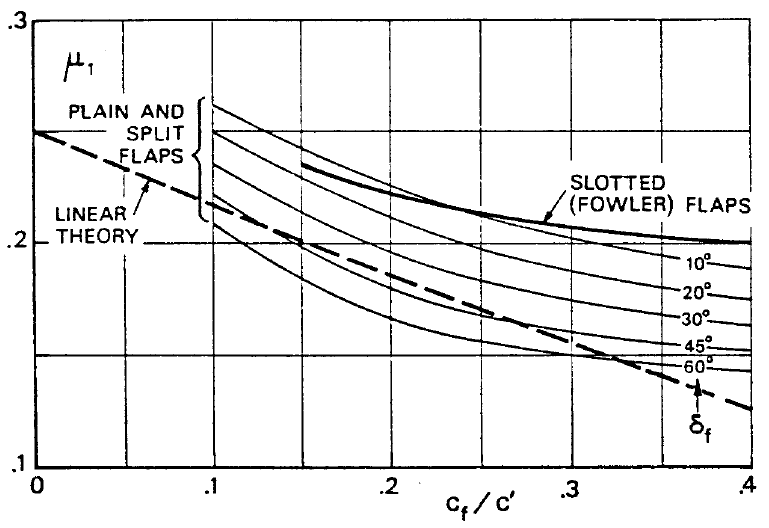
\includegraphics[width=0.7\linewidth]{Mu1_Pitching_Moment}
\caption{The pitching moment function $\mu_1$}
\label{fig:Mu1}
\end{figure}
%
The last term of the (\ref{eqn:Mu1}) is generally of a low order and can be ignored. This, together with the halving of the second term of the previous equation, leads to the following practical expression of $\upDelta C_{m_{\frac{c}{4}}}$.

\begin{equation}
\upDelta C_{m_{\frac{c}{4}}}=-\mu_1\ \upDelta C_{l\text{max}}\ \left(\dfrac{c'}{c}\right)-\dfrac{C_l}{8}\ \dfrac{c'}{c}\left(\dfrac{c'}{c}-1\right)
\label{eqn:DeltaCmPractical}
\end{equation}

\bigskip
\noindent
The obtained two-dimensional equation can, then, be converted into a three-dimensional one, which computes the pitching moment change on the entire wing, as follows.
%
\begin{equation}
\upDelta C_{M_{\frac{c}{4}}}=\mu_2\ \upDelta C_{m_{\frac{c}{4}}}+0.7\ \dfrac{\AR}{1+\frac{2}{\AR}}\ \mu_3\ \upDelta C_{l_{\text{max}}}\ \tan\Lambda_{\frac{c}{4}}
\label{eqn:DeltaCM}
\end{equation}
%
where $\upDelta C_{m_{\frac{c}{4}}}$ is the one from (\ref{eqn:DeltaCmPractical}), provide that $C_l=C_L+\upDelta C_{l\text{max}}\left(1-\frac{S_{w,f}}{S}\right)$, and the correction factors $\mu_2$ and $\mu_3$ are the one shown in figures~\ref{fig:Mu2} and~\ref{fig:Mu3}.

\bigskip
\begin{figure}[H]
\centering
\begin{minipage}{.5\textwidth}
\centering
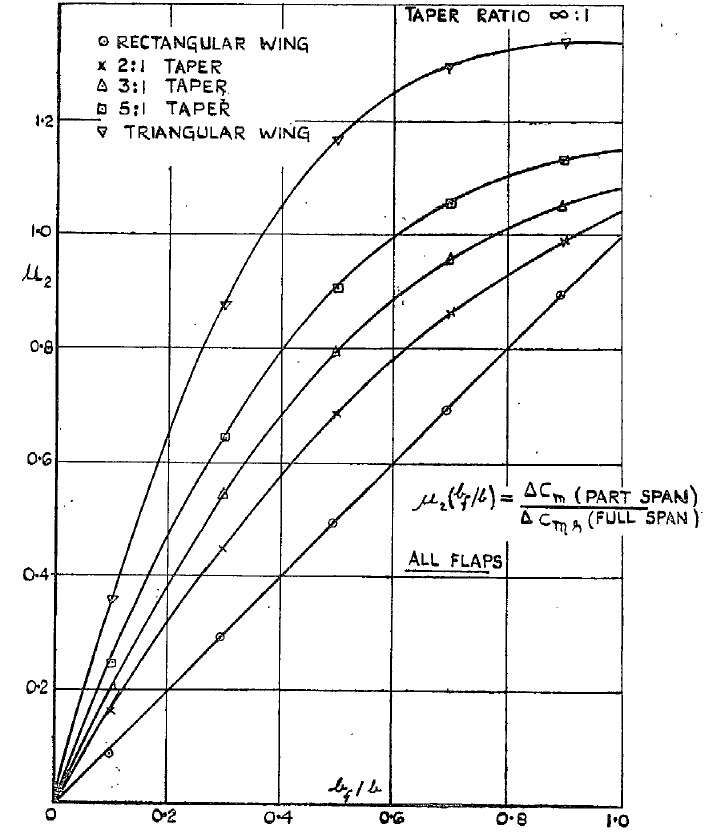
\includegraphics[width=1.1\linewidth]{Mu2_Pitching_Moment}
\captionof{figure}{The pitching moment function $\mu_2$}
\label{fig:Mu2}
\end{minipage}%
\begin{minipage}{.5\textwidth}
\centering
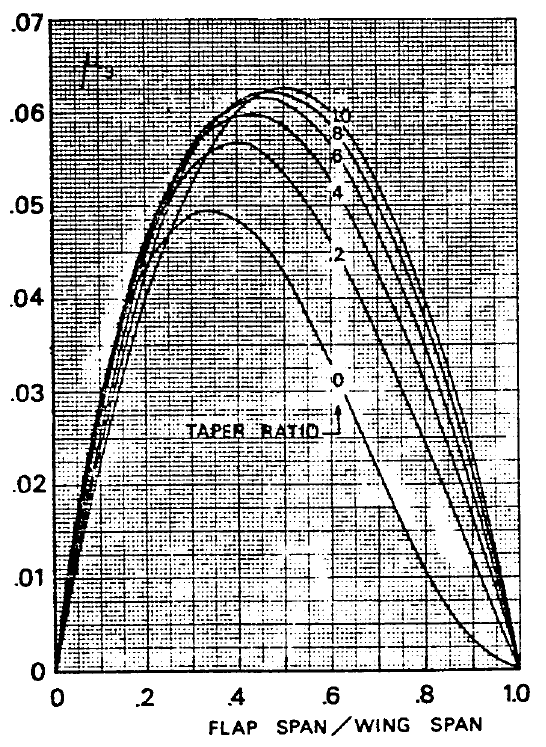
\includegraphics[width=0.94\linewidth]{Mu3_Pitching_Moment}
\captionof{figure}{The pitching moment function $\mu_3$}
\label{fig:Mu3}
\end{minipage}
\end{figure}

\noindent
Making the appropriate substitutions, the following operational formula is, finally, obtained.
%
\begin{equation}
\begin{split}
\upDelta C_{M_{\frac{c}{4}}}&=\mu_2\ \left\{-\mu_1\ \upDelta C_{L\text{max}}\ \dfrac{c'}{c}-\left[C_L+\upDelta C_{l\text{max}}\left(1-\dfrac{S_{w,f}}{S}\right)\right]\dfrac{1}{8}\ \dfrac{c'}{c}\left(\dfrac{c'}{c}-1\right)\right\}\\
&\quad+0.7\ \dfrac{\AR}{1+\frac{\AR}{2}}\ \mu_3\ \upDelta C_{l\text{max}}\ \tan\Lambda_{\frac{c}{4}}
\label{eqn:DeltaCMPractical}
\end{split}
\end{equation}
%
%------------------------- JAVA CLASS ARCHITECTURE ---------------------------
\section{Java class architecture}
\label{par:CalcHighLiftDevices}
The main purpose of this paragraph is to provide a comprehensive description of how all semi-empirical methods, presented previously, are implemented and used inside the Java class created to manage high-lift devices effects upon wings. Because of the great number of charts from which some important data have to be derived, an external database, containing all the digitized curves shown in previous paragraph figures, has been created following the procedure explained in appendix~\ref{par:Appendix1}. This database, named~\lstinline[language=Java]!HighLiftDatabase!, is then read by a dedicated class created inside the database package of~\lstinline[language=Java]!JPADCore! which name is~\lstinline[language=Java]!HighLiftDatabaseReader!; the latter, in particular, has been built up following the guideline of appendix~\ref{par:Appendix2}.

\bigskip
\noindent
Having now a powerful tool to bypass the charts reading, it's now possible to create the Java class dedicated to the management of high-lift devices effects. Since this class, named~\lstinline[language=Java]!CalcHighLiftDevices!, has to evaluate these effects on a wing, the philosophy followed in its creation suggests to relate it to the class in charge of all analysis upon a lifting surface; in particular, this class is named~\lstinline[language=Java]!LSAerodynamicsManager! and~\lstinline[language=Java]!CalcHighLiftDevices! is an inner class of it.

\bigskip
\noindent
The first component of~\lstinline[language=Java]!CalcHighLiftDevices! that has to analyzed is the constructor; the latter, used whenever an object of this class has to be created, has three main purposes:
%
\begin{enumerate}
\item Assign user's inputs to their related class fields
\item Recognize flaps types from a \gls{List} of~\lstinline[language=Java]!FlapTypeEnum! objects and link them to their typical maximum deflection value; moreover it gives them an appropriate index to be used inside~\lstinline[language=Java]!HighLiftDatabaseReader! in order to access to the specific flap type curve of the database when needed
\item Perform the preliminary calculation of the wing clean maximum lift coefficient, and of the related stalling angle of attack, using the method named~\lstinline[language=Java]!calcAlphaAndCLMax!, of the~\lstinline[language=Java]!LSAerodynamicsManager!, which accepts as input the wing mean airfoil calculated by the constructor using the method~\lstinline[language=Java]!calculateMeanAirfoil!, of a~\lstinline[language=Java]!LSAerodynamicsManager! inner class named~\lstinline[language=Java]!MeanAirfoil!, which performs the calculation of the required characteristics using influence areas method based on the three main wing airfoils (Root, Kink, Tip).   
\end{enumerate}
%
\noindent
In particular~\lstinline[language=Java]!FlapTypeEnum! is an \gls{Enum}\cite{enumAPI} of possible flaps types created inside the~\lstinline[language=Java]!JPADConfigs! package to manage in a smart and intuitive way this parameter. 
%
Furthermore it has to be noted that having the clean maximum lift coefficient, and its stalling angle of attack, calculated in the constructor allows to reduce computational cost because these heavy calculations are performed only once when the object is created; this is very useful when the user wants to calculate the lift coefficient, at a specific angle of attack on the flapped lift curve, many time, for example, during iterations.  
%
\begin{table}[!t]
\makebox[\linewidth]{
\begin{tabular}{ccc}
\toprule
\textbf{Available Flaps} & \textbf{Typical maximum deflection} & \textbf{Database index}\\
\midrule
Single slotted & 45° & 1.0 \\
Double slotted & 50° & 2.0 \\
Plain & 60° & 3.0 \\
Fowler & 40° & 4.0 \\
Triple slotted & 50° & 5.0 \\
\bottomrule
\end{tabular}
}
\caption{Summary of available flaps types with their related properties}
\label{table:AvailableFlaps}
\end{table}
%
\begin{table}[!b]
\makebox[\linewidth]{
\begin{tabular}{p{0.2\linewidth}p{0.8\linewidth}}
\toprule
\lstinline[language=Java]!theWing! & A \lstinline[language=Java]!LiftingSurface! object representing an aircraft wing \\ [0.2cm]
\lstinline[language=Java]!theConditons! & An \lstinline[language=Java]!OperatingConditions! object representing aircraft flight conditions \\  [0.2cm]
\lstinline[language=Java]!deltaFlap! & A \lstinline[language=Java]!List! of \lstinline[language=Java]!Double! arrays containing each flap deflections \\  [0.2cm]
\lstinline[language=Java]!flapType! & A \lstinline[language=Java]!List! of \lstinline[language=Java]!FlapTypeEnum! values for each flap \\  [0.2cm]
\lstinline[language=Java]!deltaSlat! & A \lstinline[language=Java]!List! of \lstinline[language=Java]!Double! values containing each slat deflections; to be set to null if there aren't slats\\  [0.2cm]
\lstinline[language=Java]!etaInFlap! & A \lstinline[language=Java]!List! of \lstinline[language=Java]!Double! values containing each flap inner dimensionless position \\  [0.2cm]
\lstinline[language=Java]!etaOutFlap! & A \lstinline[language=Java]!List! of \lstinline[language=Java]!Double! values containing each flap outer dimensionless position \\  [0.2cm]
\lstinline[language=Java]!etaInSlat! & A \lstinline[language=Java]!List! of \lstinline[language=Java]!Double! values containing each slat inner dimensionless position, to be set to null if there aren't slats \\  [0.2cm]
\lstinline[language=Java]!etaInSlat! & A \lstinline[language=Java]!List! of \lstinline[language=Java]!Double! values containing each flap outer dimensionless position, to be set to null if there aren't slats \\  [0.2cm]
\lstinline[language=Java]!cfc! & A \lstinline[language=Java]!List! of \lstinline[language=Java]!Double! values containing flap chord to airfoil chord ratios for each flap \\  [0.2cm]
\lstinline[language=Java]!csc! & A \lstinline[language=Java]!List! of \lstinline[language=Java]!Double! values containing slat chord to airfoil chord ratios for each slat, to be set to null if there aren't slats \\  [0.2cm]
\lstinline[language=Java]!leRadiusRatioSlat! & A \lstinline[language=Java]!List! of  \lstinline[language=Java]!Double! values containing \gls{acr:LER} to airfoil thickness ratios $\left(\text{LER}/t=\text{LER}/c\cdot t/c\right)$ for each slat, to be set to null if there aren't slats \\  [0.2cm]
\lstinline[language=Java]!cExtcSlat! & A \lstinline[language=Java]!List! of  \lstinline[language=Java]!Double! arrays containing extended chord to airfoil chord ratios for each slat \\ 
\bottomrule
\end{tabular}
}
\caption{~\lstinline[language=Java]!CalcHighLiftDevices! constructor input}
\label{table:CalcHighLiftConstructor}
\end{table}
%
\lstinline[language=Java]!CalcHighLiftDevices! class is also made up of three main methods each of which in charge of a specific task. 

\bigskip
\noindent
The first one is~\lstinline[language=Java]!calculateHighLiftDevicesEffects! which implements all formulas explained in paragraph~\ref{sec:theoryFlapSlat} using input data derived from the constructor, and shown in table~\ref{table:CalcHighLiftConstructor}. This method is defined~\lstinline[language=Java]!void! so that it returns nothing as output; in fact, the latter has only to provide the required calculations leaving to the user the output data retrieval using the appropriate \emph{getter} methods of which the class is provided. 

\bigskip
\noindent
The second one is~\lstinline[language=Java]!calcCLatAlphaHighLiftDevice!, which requires firstly to perform the analysis of \lstinline[language=Java]!calculateHighLiftDevicesEffects!; it calculates the lift coefficient at a given angle of attack for a wing with high-lift devices deflected. This method calculates both linear trait and non-linear trait of the curve using the NASA Blackwell method for the slope of the linear trait and a cubic interpolation for the non-linear one. 
%
In particular it sums up the effect of $\upDelta C_{L0}$ to the clean wing $C_{L0}$ in order to obtain the new value with deflected high-lift devices, then it replaces the clean wing $C_{L\alpha}$ with the new one calculated with the previous method; assuming also that the angle of attack at the end of the linear trait is taken as the mean of the old one, related to the mean airfoil, and the one calculated at the same $C_L^*$ but on the new curve, the new $C_L^*$  can be evaluated completing the calculations of the linear trait parameters. From this point on, $\upDelta C_{L\text{max}}$ and $\upDelta\alpha_{\text{stall}}$ are summed to the clean curve $C_{L\text{max}}$ and $\alpha_{\text{stall}}$ calculated into the constructor; then a cubic interpolation, starting from the end of linear trait, allows to build the non-linear one.

\bigskip
\noindent
The third, and last, method is~\lstinline[language=Java]!plotHighLiftCurve!. It is used to plot both the clean wing lift curve, both the flapped one; the first task is done by an~\lstinline[language=Java]!LSAerodynamicsManager! method named~\lstinline[language=Java]!PlotCLvsAlphaCurve!, while the second one follows the same philosophy of the previous method to calculate the lift coefficient for 30 angles of attack starting from -10° and ending at $\left(\alpha_{\text{stall}}\right)_{\text{flap}}$+2°.
%
\begin{figure}[H]
  \centering
  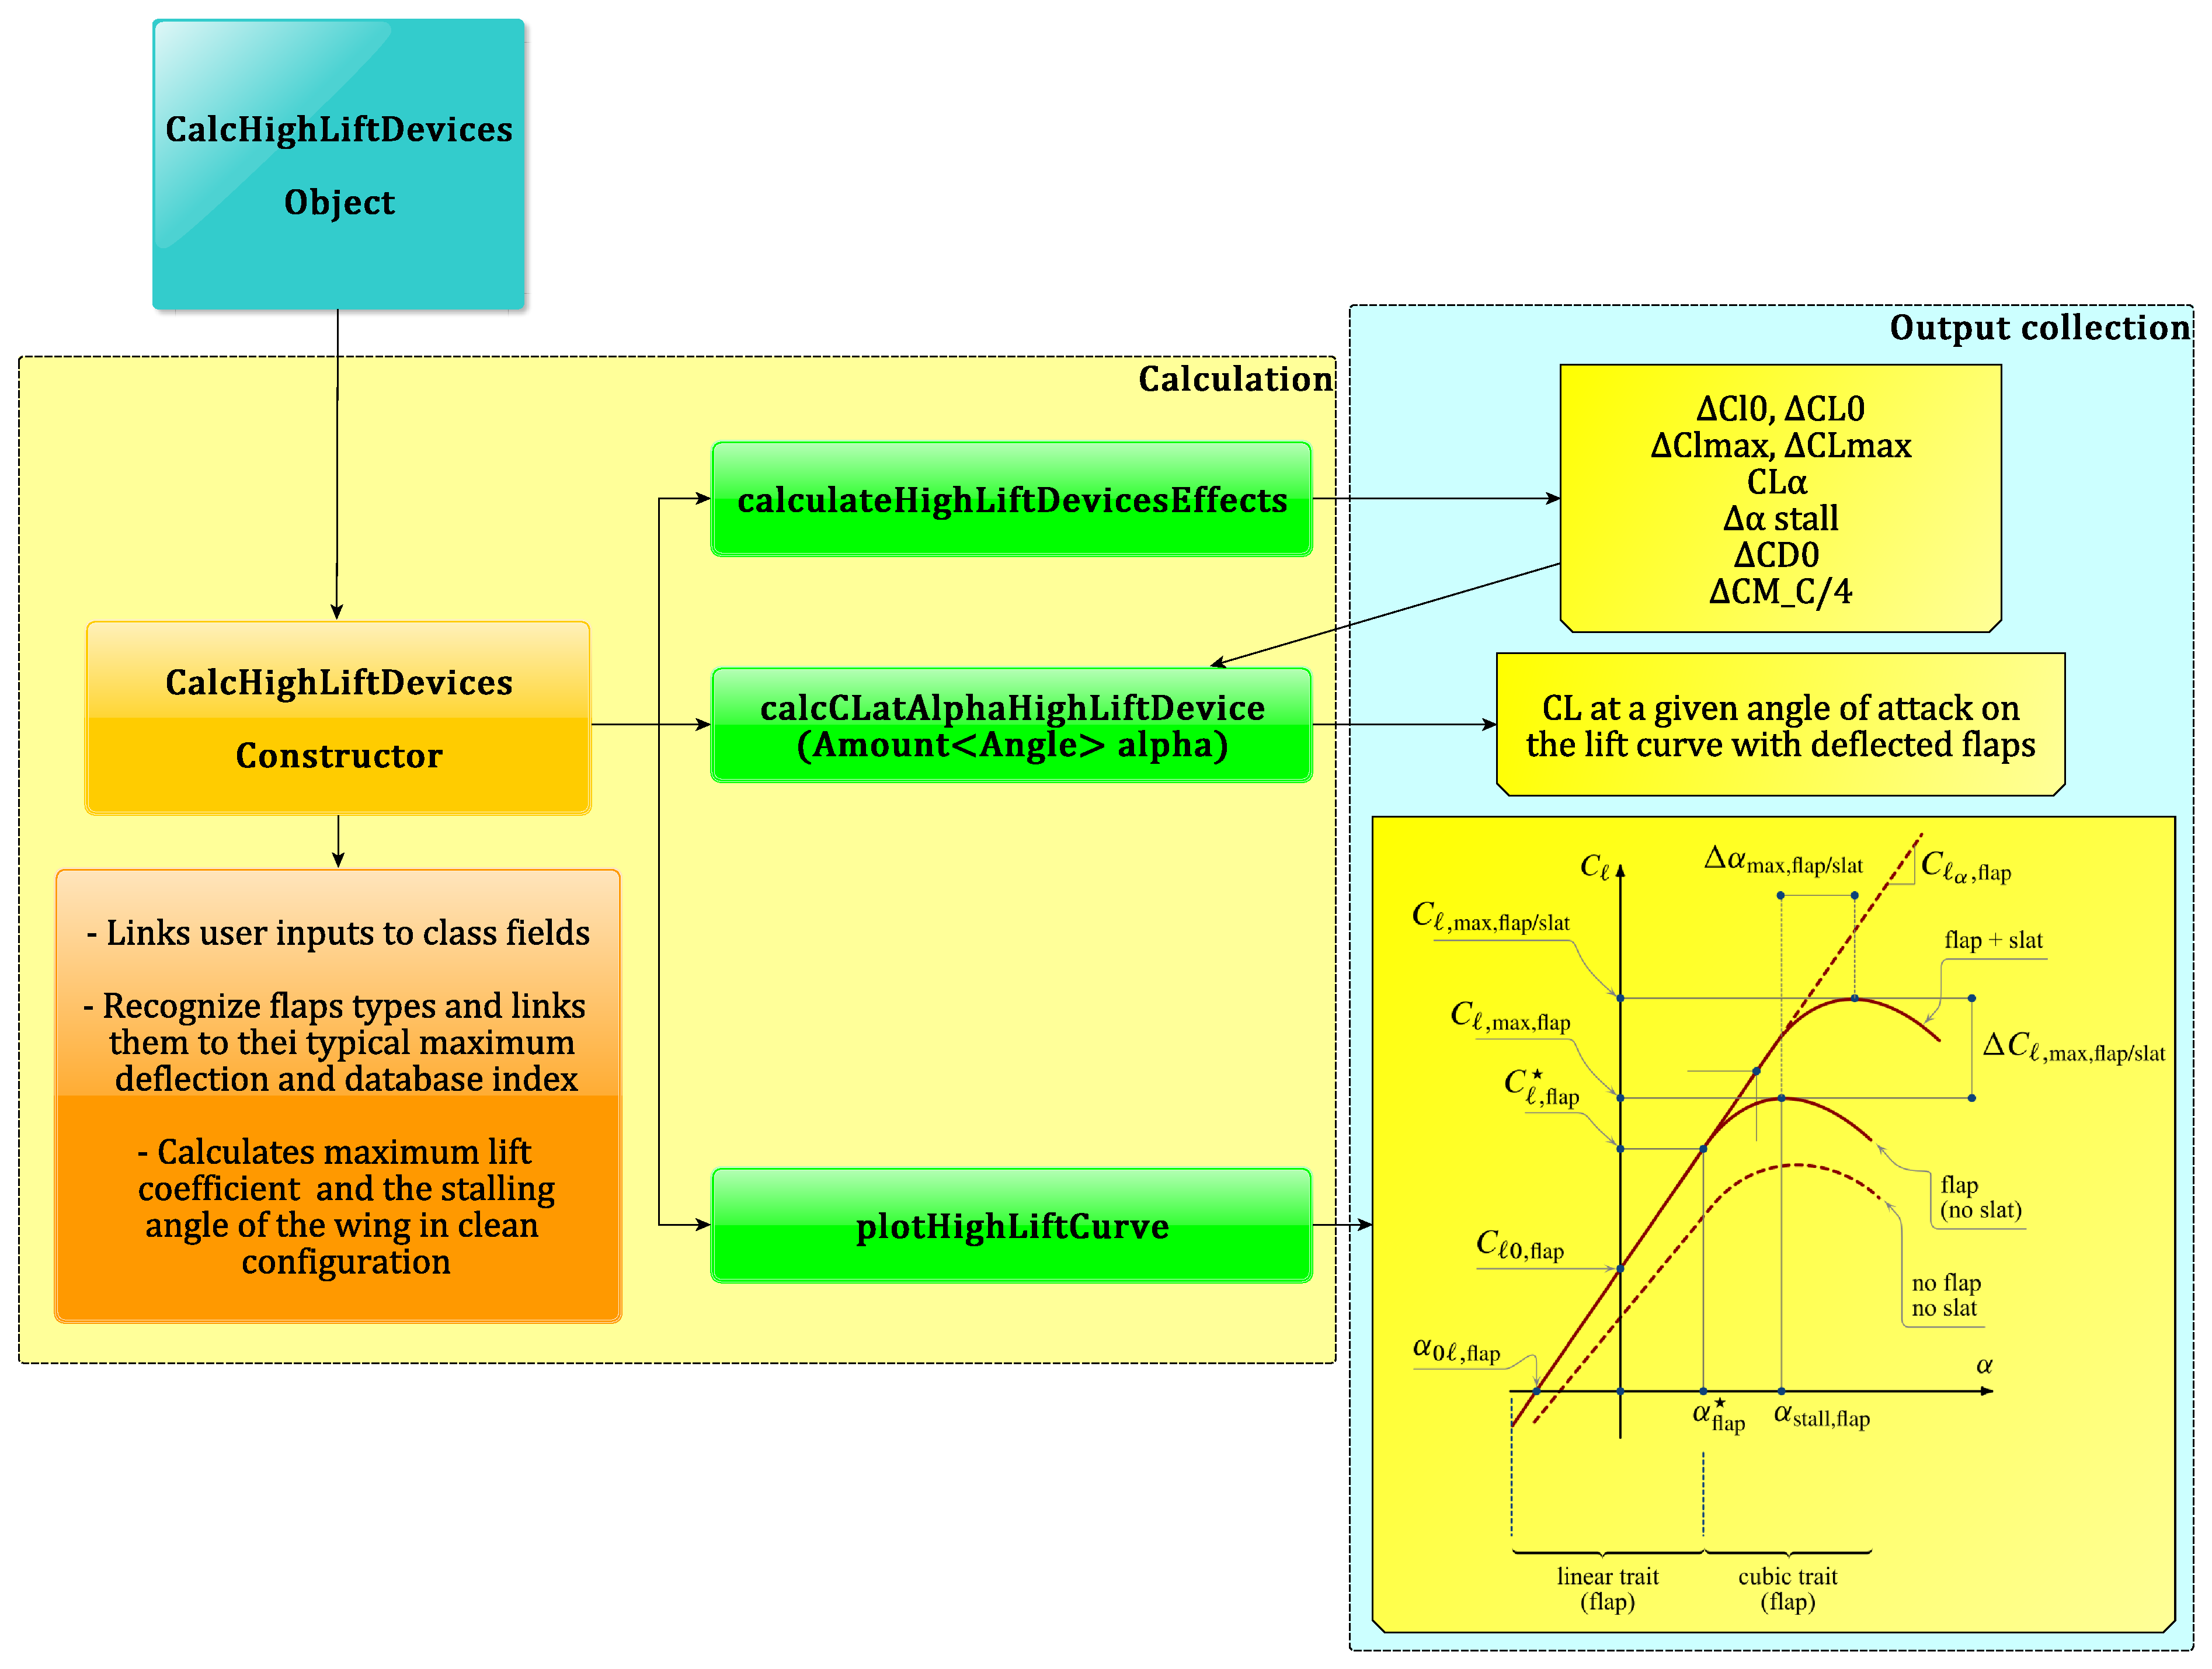
\includegraphics[width=1.07\linewidth]{HighLiftDevices_Flowchart}
  \caption{~\lstinline[language=Java]!CalcHighLiftDevices! class flowchart}
  \label{fig:CalcHighLiftFlowchart}
\end{figure}
%
%----------------------- CASE STUDY : ATR72 AND B747 -------------------------
\section{Case study: ATR-72 and B747-100B}
\label{par:CaseStudyHighLift}
The last task to be done is to show an application of the~\lstinline[language=Java]!CalcHighLiftDevices! class in order to validate the calculation performed as well as to give a useful example to a potential user developer. 
%
As in previous chapters the test will be performed using ATR-72 and B747-100B aircraft models, built up as explained in paragraph~\ref{par:DefaultAircraft}. These aircraft models doesn't have high-lift devices input data embedded, so that they have to be assigned from an external XML file; this choice has been taken because the user may want to try different high-lift devices setups without changing the aircraft model on which these latter will be applied.
%
The input XML file\cite{wiki:xml} has to provide all data from table~\ref{table:CalcHighLiftConstructor}, except for the lifting surface model and the operating condition, and it is modeled as follows.

\bigskip
\begin{lstlisting}[caption={Example of high-lift devices XML input file for the B747-100B in take-off configuration}, captionpos=b, tabsize=6, language=XML]
<input>
	<B747>
		<Flap_Number unit="">2</Flap_Number>
		<Flap1>
			<FlapType unit="">TRIPLE_SLOTTED</FlapType>
			<Cf_C unit="">0.18</Cf_C>
			<Delta_Flap1 unit="deg">5</Delta_Flap1>
			<Delta_Flap1 unit="deg">3</Delta_Flap1>
			<Delta_Flap1 unit="deg">2</Delta_Flap1>
			<Flap_inboard>0.104</Flap_inboard>
			<Flap_outboard>0.357</Flap_outboard>
		</Flap1>
		<Flap2>
			<FlapType unit="">TRIPLE_SLOTTED</FlapType>
			<Cf_C unit="">0.18</Cf_C>
			<Delta_Flap2 unit="deg">5</Delta_Flap2>
			<Delta_Flap2 unit="deg">3</Delta_Flap2>
			<Delta_Flap2 unit="deg">2</Delta_Flap2>
			<Flap_inboard unit="">0.411</Flap_inboard>
			<Flap_outboard unit="">0.636</Flap_outboard>
		</Flap2>
		<Slat1>
			<Delta_Slat unit="deg">10</Delta_Slat>
			<Cs_C unit="">0.09</Cs_C>
			<cExt_c unit="">1.1</cExt_c>
			<LEradius_c_ratio unit="">0.0097</LEradius_c_ratio>
			<Slat_inboard unit="">0.192</Slat_inboard>
			<Slat_outboard unit="">0.364</Slat_outboard>
		</Slat1>
		<Slat2>
			<Delta_Slat unit="deg">10</Delta_Slat>
			<Cs_C unit="">0.136</Cs_C>
			<cExt_c unit="">1.1</cExt_c>
			<LEradius_c_ratio unit="">0.0097</LEradius_c_ratio>
			<Slat_inboard unit="">0.414</Slat_inboard>
			<Slat_outboard unit="">0.648</Slat_outboard>
		</Slat2>
		<Slat3>
			<Delta_Slat unit="deg">10</Delta_Slat>
			<Cs_C unit="">0.187</Cs_C>
			<cExt_c unit="">1.1</cExt_c>
			<LEradius_c_ratio unit="">0.0097</LEradius_c_ratio>
			<Slat_inboard unit="">0.692</Slat_inboard>
			<Slat_outboard unit="">0.961</Slat_outboard>
		</Slat3>
	</B747>
</input>
\end{lstlisting}

\bigskip
\begin{lstlisting}[caption={Example of high-lift devices XML input file for the ATR-72 in take-off configuration}, captionpos=b, tabsize=6, language=XML]
<input>
	<ATR72>
		<Flap_Number unit="">2</Flap_Number>
		<Flap1>
			<FlapType unit="">SINGLE_SLOTTED</FlapType>
			<Cf_c unit="">0.38</Cf_c>
			<Delta_Flap1 unit="deg">20</Delta_Flap1>
			<Flap_inboard>0.08</Flap_inboard>
			<Flap_outboard>0.35</Flap_outboard>
		</Flap1>
		<Flap2>
			<FlapType unit="">SINGLE_SLOTTED</FlapType>
			<Cf_c unit="">0.38</Cf_c>
			<Delta_Flap2 unit="deg">20</Delta_Flap2>
			<Flap_inboard>0.35</Flap_inboard>
			<Flap_outboard>0.8</Flap_outboard>
		</Flap2>
	</ATR72>
</input>
\end{lstlisting}

\bigskip
\noindent
The first thing to do in order to read these data is use the Java library~\lstinline[language=Java]!args4j!; the latter allows the user to make the \gls{parsing} of the input file in order to make it available for reading inside the test class. For more information regarding this library the reader can consult~\cite{args4j}.
%
After the input file has been parsed correctly, the reading process can start. The user now has to create a \gls{List} for each input data of table~\ref{table:CalcHighLiftConstructor} and then an object of the class~\lstinline[language=Java]!JPADXmlReader!, of the~\lstinline[language=Java]!JPADCore!~\lstinline[language=Java]!standaloneutils! package, in order to manage the scan of the XML file through its methods. 

\bigskip
\begin{lstlisting}[caption={Excerpt of B747-100B test - Input data reading}, captionpos=b, tabsize=2]
	// High Lift Devices Input
	List<Double[]> deltaFlap = new ArrayList<Double[]>();
	List<FlapTypeEnum> flapType = new ArrayList<FlapTypeEnum>();
	List<Double> etaInFlap = new ArrayList<Double>();
	List<Double> etaOutFlap = new ArrayList<Double>();
	List<Double> cfc = new ArrayList<Double>();
	List<Double> deltaSlat = new ArrayList<Double>();
	List<Double> etaInSlat = new ArrayList<Double>();
	List<Double> etaOutSlat = new ArrayList<Double>();
	List<Double> csc = new ArrayList<Double>();
	List<Double> cExtcSlat = new ArrayList<Double>();
	List<Double> leRadiusSlatRatio = new ArrayList<Double>();
	// XML reading phase:
	// Arguments check
	if (args.length == 0){
		System.err.println("NO INPUT FILE GIVEN --> TERMINATING");
		return;}
	// Input file parsing
	main.theCmdLineParser.parseArgument(args);
	// Creation of the reader object
	String path = main.get_inputFile().getAbsolutePath();
	JPADXmlReader reader = new JPADXmlReader(path);
	// XML file scan through JPADXmlReader methods
	List<String> flapNumberProperty = reader.getXMLPropertiesByPath("//Flap_Number");
	int flapNumber = Integer.valueOf(flapNumberProperty.get(0));
	List<String> flapTypeProperty = reader.getXMLPropertiesByPath("//FlapType");
	List<String> cfcProperty = reader.getXMLPropertiesByPath("//Cf_C");
	List<String> deltaFlap1Property = reader.getXMLPropertiesByPath("//Delta_Flap1");
	List<String> deltaFlap2Property = reader.getXMLPropertiesByPath("//Delta_Flap2");
	List<String> etaInFlaProperty = reader.getXMLPropertiesByPath("//Flap_inboard");
	List<String> etaOutFlapProperty = 
					reader.getXMLPropertiesByPath("//Flap_outboard");
	List<String> deltaSlatProperty = reader.getXMLPropertiesByPath("//Delta_Slat");
	List<String> cscProperty = reader.getXMLPropertiesByPath("//Cs_C");
	List<String> cExtcSlatProperty = reader.getXMLPropertiesByPath("//cExt_c");
	List<String> leRadiusSlatRatioProperty = 
					reader.getXMLPropertiesByPath("//LEradius_c_ratio");
	List<String> etaInSlatProperty = reader.getXMLPropertiesByPath("//Slat_inboard");
	List<String> etaOutSlatProperty = 
					reader.getXMLPropertiesByPath("//Slat_outboard");
	// Management of the Lists of String in order to populate the previous Lists  
	// Recognizing flap type
	for(int i=0; i<flapTypeProperty.size(); i++) {
		if(flapTypeProperty.get(i).equals("SINGLE_SLOTTED"))
			flapType.add(FlapTypeEnum.SINGLE_SLOTTED);
		else if(flapTypeProperty.get(i).equals("DOUBLE_SLOTTED"))
			flapType.add(FlapTypeEnum.DOUBLE_SLOTTED);
		else if(flapTypeProperty.get(i).equals("PLAIN"))
			flapType.add(FlapTypeEnum.PLAIN);
		else if(flapTypeProperty.get(i).equals("FOWLER"))
			flapType.add(FlapTypeEnum.FOWLER);
		else if(flapTypeProperty.get(i).equals("TRIPLE_SLOTTED"))
			flapType.add(FlapTypeEnum.TRIPLE_SLOTTED);
		else {
			System.err.println("NO VALID FLAP TYPE!!");
			return;
		}
	}
	Double[] deltaFlap1Array = new Double[delta_flap1_property.size()];
	for(int i=0; i<deltaFlap1Array.length; i++)
		deltaFlap1Array[i] = Double.valueOf(deltaFlap1Property.get(i));
		Double[] deltaFlap2Array = new Double[deltaFlap2Property.size()];
	for(int i=0; i<deltaFlap1Array.length; i++)
		deltaFlap2Array[i] = Double.valueOf(deltaFlap2Property.get(i));
		deltaFlap.add(deltaFlap1Array);
	deltaFlap.add(deltaFlap2Array);
		for(int i=0; i<cfcProperty.size(); i++)
		cfc.add(Double.valueOf(cfcProperty.get(i)));
	for(int i=0; i<etaInFlapProperty.size(); i++)
		etaInFlap.add(Double.valueOf(etaInFlapProperty.get(i)));
	for(int i=0; i<etaOutFlapProperty.size(); i++)
		etaOutFlap.add(Double.valueOf(etaOutFlapProperty.get(i)));
	for(int i=0; i<deltaSlatProperty.size(); i++)
		deltaSlat.add(Double.valueOf(deltaSlatProperty.get(i)));
	for(int i=0; i<cscProperty.size(); i++)
		csc.add(Double.valueOf(cscProperty.get(i)));
	for(int i=0; i<cExtcSlatProperty.size(); i++)
		cExtcSlat.add(Double.valueOf(cExtcSlatProperty.get(i)));
	for(int i=0; i<leRadiusSlatRatioProperty.size(); i++)
		leRadiusSlatRatio.add(Double.valueOf(leRadiusSlatRatioProperty.get(i)));
	for(int i=0; i<etaInSlatProperty.size(); i++)
		etaInSlat.add(Double.valueOf(etaInSlatProperty.get(i)));
	for(int i=0; i<etaOutSlatProperty.size(); i++)
		etaOutSlat.add(Double.valueOf(etaOutSlatProperty.get(i)));
\end{lstlisting}

\bigskip
\noindent
It's important to highlight that~\lstinline[language=Java]!JPADXmlReader! methods can return an~\lstinline[language=Java]!Amount!\cite{jscienceAmount} or a~\lstinline[language=Java]!String! for each data read this way so that a post-reading management is necessary in order to have data in correct types. At this point all the required data are ready for use; now the user just have to create the object of the class~\lstinline[language=Java]!CalcHighLiftDevices! and call its methods as described in figure~\ref{fig:CalcHighLiftFlowchart}.
%
It has to be noted that, since~\lstinline[language=Java]!CalcHighLiftDevices! is a class nested into~\lstinline[language=Java]!LSAerodynamicsManager!, the creation of the required object is a little bit different from the usual; in particular an object of~\lstinline[language=Java]!LSAerodynamicsManager!, named~\lstinline[language=Java]!theLSAnalysis! in the example below, has to be created first and then the~\lstinline[language=Java]!CalcHighLiftDevices! one can be created as follows.

\bigskip
\lstset{language=Java}
\begin{lstlisting}[caption={Excerpt of B747-100B test - calculator object creation}, captionpos=b, tabsize=2]
	LSAerodynamicsManager.CalcHighLiftDevices highLiftCalculator = theLSAnalysis
					.new CalcHighLiftDevices(
							aircraft.get_wing(),
							theCondition,
							deltaFlap,
							flapType,
							deltaSlat,
							eta_in_flap,
							eta_out_flap,
							eta_in_slat,
							eta_out_slat,
							cf_c,
							cs_c,
							leRadius_c_slat,
							cExt_c_slat
							);
\end{lstlisting}

\bigskip
\noindent
In conclusion, numerical and graphical results of the described tests, applied to the two aircraft mentioned at the beginning of paragraph, are shown.
%
\begin{figure}[H]
\centering
%CL alpha Wing High Lift
\begin{tikzpicture}

\begin{axis}[
width=0.8\textwidth,
height=0.5\textheight,
scaled ticks=false, tick label style={/pgf/number format/fixed},
xmin=-15.0,
xmax=25,
xlabel={$alpha_w$ ($\deg$)},
xmajorgrids,
ymin=-1,
ymax=2.5,
ylabel={C\textsubscript{L}},
ymajorgrids,
legend style={at={(0.03,0.85)},anchor=west,draw=black,fill=white,legend cell align=left},
legend entries = {Clean\\Flap@TO\\}
]

\addplot [
color=black,
densely dashed
]
table[row sep=crcr]{
-10.0	-0.8052979685827285\\
-9.23559843465475	-0.7355525089447045\\
-8.471196869309502	-0.6658070493066807\\
-7.7067953039642525	-0.5960615896686566\\
-6.942393738619003	-0.5263161300306327\\
-6.177992173273754	-0.45657067039260846\\
-5.413590607928505	-0.38682521075458454\\
-4.649189042583256	-0.31707975111656045\\
-3.8847874772380067	-0.24733429147853653\\
-3.1203859118927575	-0.17758883184051244\\
-2.3559843465475083	-0.10784337220248841\\
-1.591582781202259	-0.03809791256446435\\
-0.8271812158570095	0.03164754707355967\\
-0.06277965051176015	0.10139300671158373\\
0.7016219148334892	0.17113846634960778\\
1.4660234801787386	0.24088392598763184\\
2.230425045523988	0.31062938562565584\\
2.9948266108692376	0.38037484526367993\\
3.759228176214487	0.450120304901704\\
4.523629741559736	0.519865764539728\\
5.288031306904985	0.589611224177752\\
6.052432872250234	0.659356683815776\\
6.8168344375954835	0.7291021434538\\
7.581236002940733	0.7988476030918241\\
8.345637568285982	0.8685930627298482\\
9.110039133631231	0.938338522367872\\
9.87444069897648	1.0082217099765014\\
10.63884226432173	1.0796203878198667\\
11.403243829666978	1.1515248638118902\\
12.167645395012228	1.2221932455843425\\
12.932046960357477	1.289883640768993\\
13.696448525702726	1.352854156997613\\
14.460850091047975	1.409362901901972\\
15.225251656393224	1.4576679831138426\\
15.989653221738473	1.4960275082649925\\
16.754054787083724	1.5226995849871936\\
17.518456352428974	1.5359423209122145\\
18.282857917774223	1.5340138236718266\\
19.047259483119472	1.5151722008978004\\
19.811661048464728	1.4776755602219067\\
};

\addplot [
color=black,
solid
]
table[row sep=crcr]{
-13.0	-0.27935687283971644\\
-12.3371824964394	-0.21841084753104578\\
-11.6743649928788	-0.15746482222237534\\
-11.0115474893182	-0.09651879691370491\\
-10.3487299857576	-0.03557277160503436\\
-9.685912482197	0.02537325370363608\\
-9.0230949786364	0.08631927901230674\\
-8.3602774750758	0.14726530432097706\\
-7.6974599715152	0.20821132962964772\\
-7.034642467954599	0.26915735493831827\\
-6.371824964393999	0.33010338024698893\\
-5.709007460833398	0.3910494055556595\\
-5.046189957272797	0.4519954308643301\\
-4.383372453712196	0.5129414561730006\\
-3.7205549501515955	0.5738874814816712\\
-3.057737446590995	0.6348335067903419\\
-2.394919943030394	0.6957795320990124\\
-1.7321024394697933	0.756725557407683\\
-1.0692849359091925	0.8176715827163537\\
-0.40646743234859173	0.8786176080250242\\
0.25635007121200903	0.9395636333336947\\
0.9191675747726098	1.0005096586423654\\
1.5819850783332106	1.0614556839510358\\
2.2448025818938113	1.1224017092597065\\
2.907620085454412	1.1833477345683772\\
3.570437589015013	1.2442937598770478\\
4.233255092575614	1.3052397851857183\\
4.896072596136214	1.366185810494389\\
5.558890099696815	1.427560580275692\\
6.221707603257416	1.4910894361240157\\
6.884525106818017	1.5561917452948077\\
7.547342610378617	1.6219810924290692\\
8.210160113939217	1.6875710621678006\\
8.872977617499817	1.7520752391520038\\
9.535795121060417	1.814607208022679\\
10.198612624621017	1.8742805534208276\\
10.861430128181617	1.93020885998745\\
11.524247631742217	1.981505712363548\\
12.187065135302817	2.027284695190122\\
12.849882638863416	2.0666593931081736\\
13.512700142424016	2.0987433907587025\\
14.175517645984616	2.1226502727827112\\
14.838335149545216	2.1374936238211997\\
15.501152653105816	2.1423870285151687\\
16.163970156666416	2.13644407150562\\
16.826787660227016	2.1187783374335543\\
17.489605163787616	2.088503410939973\\
18.152422667348215	2.0447328766658757\\
18.815240170908815	1.9865803192522646\\
19.47805767446944	1.9131593233401376\\
};
\end{axis}
\end{tikzpicture}%

\caption{ATR-72 lift curve with and without flaps deflected in take-off configuration}
\label{fig:FlapATR}
\end{figure}

\bigskip
\lstset{language=Java}
\begin{lstlisting}[caption={ATR-72 test results}, captionpos=b, tabsize=2]
deltaCl0_flap = 2.263493753740178
deltaCL0_flap = 0.7527037903308272
deltaClmax_flap = 1.2122379635109801
deltaCLmax_flap = 0.5249013462746028
CLalpha_new = 0.09139075701076349 (1/deg)
deltaCD = 0.017691818247996084
deltaCMc_4 = -0.12100839839572519
-----------CLEAN-------------- 
 alpha max 18.456192298464735 (deg)
 CL max 1.5842572610046424
 CL star 0.9782965664494722
 CL alpha 5.189644003702157 (1/rad)
 -----------HIGH LIFT-------------- 
 alpha max 15.81817306525097 (deg)
 CL max 2.1091586072792454
 CL star 1.3586008009300286
 CL alpha 5.236690376716748 (1/rad)
\end{lstlisting}
%
\begin{figure}[H]
\centering
%CL alpha Wing High Lift
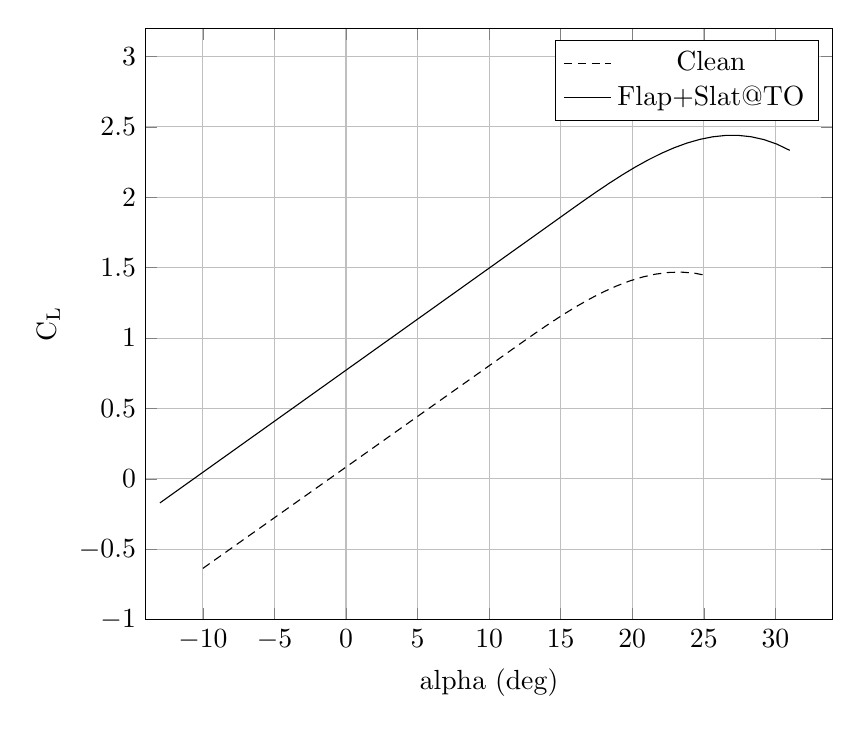
\begin{tikzpicture}

\begin{axis}[
width=0.85\textwidth,
height=0.75\textwidth,
scaled ticks=false, tick label style={/pgf/number format/fixed},
xmin=-14.0,
xmax=34,
xlabel={alpha ($\deg$)},
xmajorgrids,
ymin=-1,
ymax=3.2,
ylabel={C\textsubscript{L}},
ymajorgrids,
legend entries = {Clean\\Flap+Slat@TO\\}
]

\addplot [
color=black,
densely dashed
]
table[row sep=crcr]{
-10.0	-0.6352658757762881\\
-9.096634542963105	-0.5702848523339756\\
-8.193269085926211	-0.5053038288916633\\
-7.289903628889317	-0.44032280544935076\\
-6.386538171852424	-0.3753417820070383\\
-5.48317271481553	-0.3103607585647258\\
-4.579807257778636	-0.24537973512241334\\
-3.6764418007417428	-0.1803987116801009\\
-2.773076343704849	-0.11541768823778845\\
-1.8697108866679555	-0.05043666479547601\\
-0.9663454296310617	0.014544358646836467\\
-0.06297997259416799	0.07952538208914893\\
0.8403854844427258	0.14450640553146138\\
1.7437509414796195	0.20948742897377387\\
2.647116398516513	0.2744684524160863\\
3.550481855553407	0.33944947585839874\\
4.453847312590301	0.40443049930071123\\
5.3572127696271945	0.46941152274302367\\
6.260578226664088	0.534392546185336\\
7.163943683700982	0.5993735696276485\\
8.067309140737876	0.6643545930699613\\
8.97067459777477	0.7293356165122736\\
9.874040054811665	0.7943166399545861\\
10.77740551184856	0.8593689436002814\\
11.680770968885454	0.9246322172626655\\
12.584136425922349	0.9894724954476011\\
13.487501882959243	1.0531586305634764\\
14.390867339996138	1.1149594750186804\\
15.294232797033033	1.174143881221601\\
16.197598254069927	1.2299807015806272\\
17.10096371110682	1.2817387885041476\\
18.004329168143716	1.3286869944005508\\
18.90769462518061	1.3700941716782251\\
19.811060082217505	1.4052291727455593\\
20.7144255392544	1.433360850010942\\
21.617790996291294	1.4537580558827616\\
22.52115645332819	1.4656896427694075\\
23.424521910365083	1.4684244630792667\\
24.327887367401978	1.4612313692207288\\
25.231252824438855	1.4433792136021832\\
};

\addplot [
color=black,
solid
]
table[row sep=crcr]{
-13.0	-0.17033511677697522\\
-12.101999963568241	-0.10525071989031021\\
-11.203999927136483	-0.04016632300364531\\
-10.305999890704724	0.024918073883019698\\
-9.407999854272965	0.0900024707696847\\
-8.509999817841207	0.15508686765634938\\
-7.611999781409449	0.2201712645430144\\
-6.713999744977691	0.28525566142967906\\
-5.815999708545934	0.3503400583163439\\
-4.917999672114176	0.41542445520300886\\
-4.019999635682418	0.4805088520896737\\
-3.1219995992506604	0.5455932489763384\\
-2.2239995628189027	0.6106776458630034\\
-1.3259995263871447	0.6757620427496682\\
-0.4279994899553867	0.7408464396363331\\
0.47000054647637124	0.805930836522998\\
1.3680005829081292	0.8710152334096628\\
2.266000619339887	0.9360996302963277\\
3.1640006557716447	1.0011840271829926\\
4.062000692203402	1.0662684240696574\\
4.96000072863516	1.1313528209563222\\
5.858000765066918	1.1964372178429872\\
6.756000801498676	1.261521614729652\\
7.654000837930433	1.3266060116163167\\
8.552000874362191	1.3916904085029818\\
9.45000091079395	1.4567748053896468\\
10.348000947225708	1.5218592022763118\\
11.246000983657467	1.5869435991629763\\
12.144001020089226	1.6520279960496413\\
13.042001056520984	1.7171123929363064\\
13.940001092952743	1.7821967898229714\\
14.838001129384502	1.847444575736119\\
15.73600116581626	1.9127524597409153\\
16.63400120224802	1.9774072900626951\\
17.532001238679776	2.040685925175604\\
18.430001275111533	2.1018652235537854\\
19.32800131154329	2.1602220436713826\\
20.226001347975046	2.215033244002541\\
21.124001384406803	2.265575683021404\\
22.02200142083856	2.311126219202114\\
22.920001457270317	2.350961711018817\\
23.818001493702074	2.3843590169456563\\
24.71600153013383	2.4105949954567745\\
25.614001566565587	2.428946505026318\\
26.512001602997344	2.4386904041284283\\
27.4100016394291	2.4391035512372525\\
28.308001675860858	2.4294628048269304\\
29.206001712292615	2.4090450233716103\\
30.10400174872437	2.377127065345433\\
31.00200178515614	2.332985789222543\\
};
\end{axis}
\end{tikzpicture}%

\caption{B747-100B lift curve with and without flaps and slats deflected in take-off configuration}
\label{fig:FlapATR}
\end{figure}

\bigskip
\lstset{language=Java}
\begin{lstlisting}[caption={B747-100B test results}, captionpos=b, tabsize=2]
deltaCl0_flap = 1.042568723557796
deltaCL0_flap = 0.2003564365099298
deltaClmax_flap = 0.1414975497068864
deltaCLmax_flap = 0.046423506957770616
deltaClmax_slat = 1.270544480012824
deltaCLmax_slat = 0.4010166637261424
CLalpha_new = 0.07307826951197416 (1/deg)
deltaCD = 0.001877785467928246
deltaCMc_4 = -0.01156502154181518
 -----------CLEAN-------------- 
 alpha max 21.588846207012903 (deg)
 CL max 1.4615744853062498
 CL star 0.8263686942120971
 CL alpha 4.121408852511741 (1/rad)
 -----------HIGH LIFT-------------- 
 alpha max 24.766400107580708 (deg)
 CL max 1.9160894563221245
 CL star 1.2636473543834792
 CL alpha 4.187384843036119 (1/rad)
\end{lstlisting}
%
\subsection{Sensibility analysis}
%
In this subsection it's shown how the~\lstinline[language=Java]!CalcHighLiftDevices! class behaves with different input parameters. In particular it is interesting to analyze the effect on the lift curve of the following input data.
%
\begin{itemize}
\item Trailing edge devices deflection $\delta_f$
\item Trailing edge devices chord ratio $\frac{c_f}{c}$ 
\item Devices type 
\item Leading edge devices deflection $\delta_s$
\end{itemize}
%
For each of these, one parameter will be modified leaving unchanged the other three. The following figures show these effects on the B747-100B having assumed as a baseline the following condition.
%
\begin{table}[H]
\makebox[\linewidth]{
\begin{tabular}{lcc|lcc}
\toprule
\textbf{Input data} &\textbf{} & \textbf{} &\textbf{Baseline results} &\textbf{}  & \textbf{} \\
\midrule
\textbf{Variables} & \textbf{} & \textbf{Value} & \textbf{Variables} & \textbf{} & \textbf{Value}\\
\midrule
$\delta_f$ &  \textbf{} & 30°  & $C_{L\text{max}}$ &  \textbf{} & 2.55 \\
$\frac{c_f}{c}$ &  \textbf{} & 0.18 & $\alpha_{\text{max}}$ &  \textbf{} & 28° \\
Trailing edge devices type &  \textbf{} & Triple Slotted & \textbf{ } &  \textbf{} & \textbf{} \\
$\delta_s$ &  \textbf{} & 15° & \textbf{ } &  \textbf{} & \textbf{} \\
\bottomrule
\end{tabular}
}
\caption{Summary of the baseline input data and results}
\end{table}
%
\begin{figure}[H]
\centering
%CL alpha high lift WING
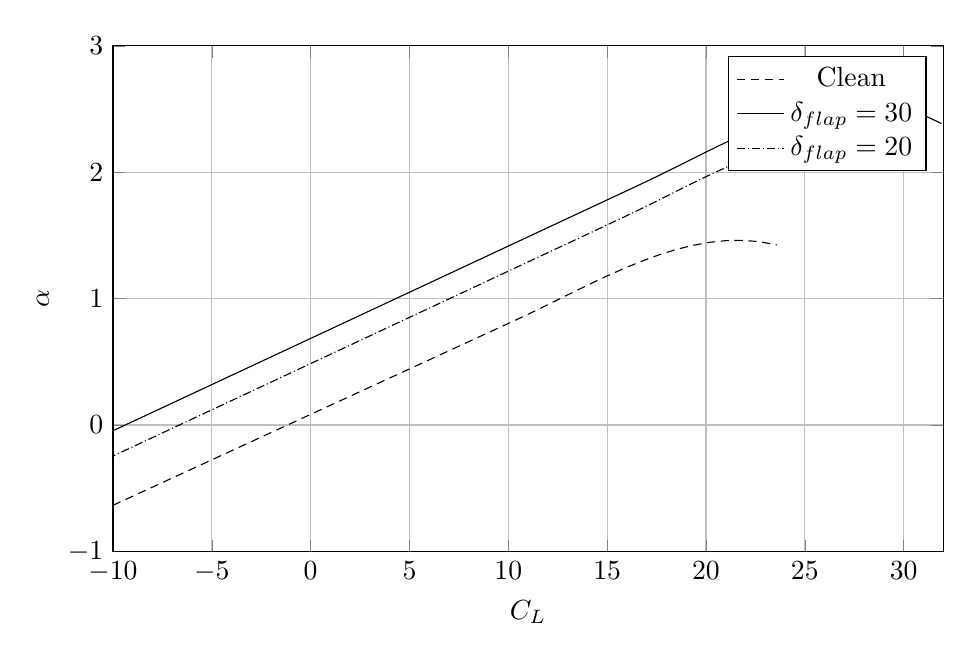
\begin{tikzpicture}

\begin{axis}[
width=\textwidth,
height=0.66\textwidth,
scaled ticks=false, tick label style={/pgf/number format/fixed},
xmin=-10,
xmax=32,
xlabel={$C_L$},
xmajorgrids,
ymin=-1,
ymax=3,
ylabel={$\alpha$},
ymajorgrids,
legend entries = {Clean\\$\delta_{\text{flap}}=\SI{30}{\degree}$\\$\delta_{\text{flap}}=\SI{20}{\degree}$\\}]

\addplot [
color=black,
densely dashed
]
table[row sep=crcr]{
-10.0	-0.6352658757762881\\
-9.138747533153515	-0.5733141304422674\\
-8.27749506630703	-0.5113623851082468\\
-7.416242599460545	-0.4494106397742259\\
-6.55499013261406	-0.38745889444020537\\
-5.693737665767576	-0.3255071491061846\\
-4.832485198921091	-0.26355540377216397\\
-3.9712327320746064	-0.20160365843814332\\
-3.1099802652281214	-0.13965191310412253\\
-2.2487277983816365	-0.0777001677701018\\
-1.3874753315351516	-0.015748422436081128\\
-0.5262228646886667	0.04620332289793959\\
0.3350296021578181	0.1081550682319603\\
1.1962820690043028	0.170106813565981\\
2.0575345358507877	0.2320585589000017\\
2.9187870026972726	0.2940103042340224\\
3.7800394695437576	0.35596204956804306\\
4.6412919363902425	0.4179137949020638\\
5.502544403236727	0.4798655402360845\\
6.3637968700832115	0.5418172855701053\\
7.225049336929696	0.6037690309041259\\
8.08630180377618	0.6657207762381466\\
8.947554270622666	0.7276725215721672\\
9.808806737469151	0.7896242669061881\\
10.670059204315637	0.8518371764996678\\
11.531311671162122	0.9162438895867622\\
12.392564138008607	0.9822400768700835\\
13.253816604855093	1.0485942706393496\\
14.115069071701578	1.1140750031842797\\
14.976321538548063	1.1774508067945915\\
15.837574005394549	1.2374902137600041\\
16.698826472241034	1.2929617563702362\\
17.560078939087518	1.3426339669150065\\
18.421331405934	1.385275377684033\\
19.282583872780485	1.4196545209670353\\
20.14383633962697	1.4445399290537297\\
21.005088806473452	1.4587001342338382\\
21.866341273319936	1.4609036687970764\\
22.72759374016642	1.4499190650331637\\
23.588846207012903	1.4245148552318199\\
};

\addplot [
color=black,
solid
]
table[row sep=crcr]{
-13.0	-0.26471729340342076\\
-12.08342596402438	-0.19775658131163865\\
-11.16685192804876	-0.13079586921985664\\
-10.250277892073141	-0.06383515712807453\\
-9.333703856097522	0.0031255549637075886\\
-8.417129820121902	0.07008626705548959\\
-7.500555784146282	0.1370469791472717\\
-6.583981748170663	0.20400769123905388\\
-5.667407712195043	0.27096840333083594\\
-4.750833676219424	0.33792911542261805\\
-3.834259640243804	0.4048898275144001\\
-2.9176856042681845	0.47185053960618223\\
-2.001111568292565	0.5388112516979643\\
-1.0845375323169453	0.6057719637897464\\
-0.1679634963413258	0.6727326758815285\\
0.7486105396342937	0.7396933879733105\\
1.665184575609913	0.8066541000650926\\
2.5817586115855327	0.8736148121568746\\
3.4983326475611523	0.9405755242486568\\
4.414906683536771	1.0075362363404388\\
5.331480719512391	1.074496948432221\\
6.248054755488011	1.141457660524003\\
7.16462879146363	1.208418372615785\\
8.081202827439249	1.2753790847075672\\
8.997776863414868	1.3423397967993491\\
9.914350899390488	1.4093005088911315\\
10.830924935366108	1.4762612209829133\\
11.747498971341727	1.5432219330746955\\
12.664073007317347	1.6101826451664776\\
13.580647043292966	1.6771433572582595\\
14.497221079268586	1.7441040693500414\\
15.413795115244206	1.8110647814418237\\
16.330369151219823	1.8780254935336056\\
17.24694318719544	1.9457429346696347\\
18.16351722317106	2.0160514914549474\\
19.080091259146677	2.0876763179934232\\
19.996665295122295	2.1591107771941327\\
20.913239331097913	2.22884823196615\\
21.82981336707353	2.295382045218546\\
22.746387403049148	2.3572055798603926\\
23.662961439024766	2.412812198800762\\
24.579535475000384	2.4606952649487277\\
25.496109510976	2.499348141213361\\
26.41268354695162	2.527264190503734\\
27.329257582927237	2.54293677572892\\
28.245831618902855	2.5448592597979895\\
29.162405654878473	2.5315250056200145\\
30.07897969085409	2.5014273761040715\\
30.99555372682971	2.453059734159225\\
31.912127762805355	2.3849154426945485\\
};

\addplot [
color=black,
densely dashdotted
]
table[row sep=crcr]{
-13.0	-0.46511040124033803\\
-12.102414036342138	-0.39945935857985265\\
-11.204828072684275	-0.3338083159193674\\
-10.307242109026413	-0.268157273258882\\
-9.409656145368551	-0.20250623059839684\\
-8.512070181710689	-0.13685518793791146\\
-7.6144842180528265	-0.0712041452774263\\
-6.716898254394964	-0.00555310261694103\\
-5.819312290737102	0.060097940043544296\\
-4.92172632707924	0.12574898270402957\\
-4.0241403634213775	0.19140002536451484\\
-3.1265543997635152	0.2570510680250001\\
-2.228968436105653	0.32270211068548543\\
-1.3313824724477907	0.3883531533459707\\
-0.4337965087899285	0.454004196006456\\
0.46378945486793377	0.5196552386669413\\
1.361375418525796	0.5853062813274266\\
2.2589613821836583	0.6509573239879118\\
3.1565473458415205	0.7166083666483971\\
4.054133309499383	0.7822594093088824\\
4.951719273157245	0.8479104519693677\\
5.849305236815107	0.9135614946298529\\
6.7468912004729695	0.9792125372903382\\
7.644477164130832	1.0448635799508235\\
8.542063127788694	1.110514622611309\\
9.439649091446556	1.176165665271794\\
10.337235055104419	1.2418167079322795\\
11.23482101876228	1.3074677505927645\\
12.132406982420143	1.37311879325325\\
13.029992946078005	1.4387698359137353\\
13.927578909735868	1.5044208785742206\\
14.82516487339373	1.5700719212347054\\
15.722750837051592	1.6357232027845487\\
16.620336800709453	1.7030037510623899\\
17.517922764367313	1.772515335414341\\
18.415508728025173	1.8428413254947649\\
19.313094691683034	1.9125650909580187\\
20.210680655340894	1.980270001458467\\
21.108266618998755	2.044539426650471\\
22.005852582656615	2.1039567361883886\\
22.903438546314476	2.1571052997265836\\
23.801024509972336	2.2025684869194144\\
24.698610473630197	2.2389296674212433\\
25.596196437288057	2.2647722108864334\\
26.493782400945918	2.2786794869693408\\
27.391368364603778	2.279234865324331\\
28.28895432826164	2.265021715605763\\
29.1865402919195	2.234623407467997\\
30.08412625557736	2.186623310565393\\
30.981712219235252	2.1196047945523135\\
};
\end{axis}
\end{tikzpicture}%

\caption{Effects of different $\delta_f$ upon the lift curve of the B747-100B with $\frac{c_f}{c}=0.18$, Triple slotted flaps and $\delta_s=\SI{15}{\degree}$}
\end{figure}
%
\begin{figure}[H]
\centering
%CL alpha high lift WING
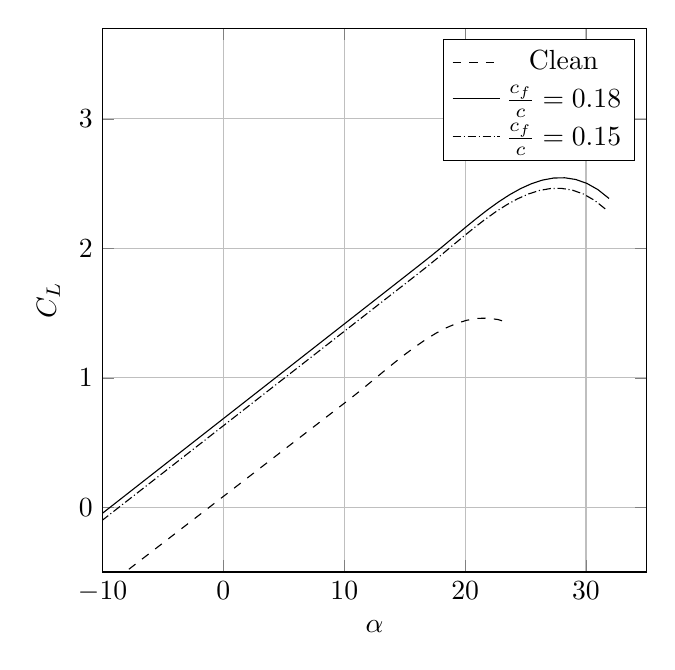
\begin{tikzpicture}

\begin{axis}[
width=0.7\textwidth,
height=0.7\textwidth,
scaled ticks=false, tick label style={/pgf/number format/fixed},
xmin=-10,
xmax=35,
xlabel={$\alpha$},
xmajorgrids,
ymin=-0.5,
ymax=3.7,
ylabel={$C_L$},
ymajorgrids,
legend entries = {Clean\\$\frac{c_f}{c}=0.18$\\$\frac{c_f}{c}=0.15$\\}]

\addplot [
color=black,
dashed
]
table[row sep=crcr]{
-10.0	-0.6352658757762881\\
-9.138747533153515	-0.5733141304422674\\
-8.27749506630703	-0.5113623851082468\\
-7.416242599460545	-0.4494106397742259\\
-6.55499013261406	-0.38745889444020537\\
-5.693737665767576	-0.3255071491061846\\
-4.832485198921091	-0.26355540377216397\\
-3.9712327320746064	-0.20160365843814332\\
-3.1099802652281214	-0.13965191310412253\\
-2.2487277983816365	-0.0777001677701018\\
-1.3874753315351516	-0.015748422436081128\\
-0.5262228646886667	0.04620332289793959\\
0.3350296021578181	0.1081550682319603\\
1.1962820690043028	0.170106813565981\\
2.0575345358507877	0.2320585589000017\\
2.9187870026972726	0.2940103042340224\\
3.7800394695437576	0.35596204956804306\\
4.6412919363902425	0.4179137949020638\\
5.502544403236727	0.4798655402360845\\
6.3637968700832115	0.5418172855701053\\
7.225049336929696	0.6037690309041259\\
8.08630180377618	0.6657207762381466\\
8.947554270622666	0.7276725215721672\\
9.808806737469151	0.7896242669061881\\
10.670059204315637	0.8518371764996678\\
11.531311671162122	0.9162438895867622\\
12.392564138008607	0.9822400768700835\\
13.253816604855093	1.0485942706393496\\
14.115069071701578	1.1140750031842797\\
14.976321538548063	1.1774508067945915\\
15.837574005394549	1.2374902137600041\\
16.698826472241034	1.2929617563702362\\
17.560078939087518	1.3426339669150065\\
18.421331405934	1.385275377684033\\
19.282583872780485	1.4196545209670353\\
20.14383633962697	1.4445399290537297\\
21.005088806473452	1.4587001342338382\\
21.866341273319936	1.4609036687970764\\
22.72759374016642	1.4499190650331637\\
23.588846207012903	1.4245148552318199\\
};

\addplot [
color=black,
solid
]
table[row sep=crcr]{
-13.0	-0.26471729340342076\\
-12.08342596402438	-0.19775658131163865\\
-11.16685192804876	-0.13079586921985664\\
-10.250277892073141	-0.06383515712807453\\
-9.333703856097522	0.0031255549637075886\\
-8.417129820121902	0.07008626705548959\\
-7.500555784146282	0.1370469791472717\\
-6.583981748170663	0.20400769123905388\\
-5.667407712195043	0.27096840333083594\\
-4.750833676219424	0.33792911542261805\\
-3.834259640243804	0.4048898275144001\\
-2.9176856042681845	0.47185053960618223\\
-2.001111568292565	0.5388112516979643\\
-1.0845375323169453	0.6057719637897464\\
-0.1679634963413258	0.6727326758815285\\
0.7486105396342937	0.7396933879733105\\
1.665184575609913	0.8066541000650926\\
2.5817586115855327	0.8736148121568746\\
3.4983326475611523	0.9405755242486568\\
4.414906683536771	1.0075362363404388\\
5.331480719512391	1.074496948432221\\
6.248054755488011	1.141457660524003\\
7.16462879146363	1.208418372615785\\
8.081202827439249	1.2753790847075672\\
8.997776863414868	1.3423397967993491\\
9.914350899390488	1.4093005088911315\\
10.830924935366108	1.4762612209829133\\
11.747498971341727	1.5432219330746955\\
12.664073007317347	1.6101826451664776\\
13.580647043292966	1.6771433572582595\\
14.497221079268586	1.7441040693500414\\
15.413795115244206	1.8110647814418237\\
16.330369151219823	1.8780254935336056\\
17.24694318719544	1.9457429346696347\\
18.16351722317106	2.0160514914549474\\
19.080091259146677	2.0876763179934232\\
19.996665295122295	2.1591107771941327\\
20.913239331097913	2.22884823196615\\
21.82981336707353	2.295382045218546\\
22.746387403049148	2.3572055798603926\\
23.662961439024766	2.412812198800762\\
24.579535475000384	2.4606952649487277\\
25.496109510976	2.499348141213361\\
26.41268354695162	2.527264190503734\\
27.329257582927237	2.54293677572892\\
28.245831618902855	2.5448592597979895\\
29.162405654878473	2.5315250056200145\\
30.07897969085409	2.5014273761040715\\
30.99555372682971	2.453059734159225\\
31.912127762805355	2.3849154426945485\\
};

\addplot [
color=black,
densely dashdotted
]
table[row sep=crcr]{
-13.0	-0.31731279095342413\\
-12.089623276578571	-0.25096631959536175\\
-11.179246553157142	-0.18461984823729927\\
-10.268869829735713	-0.11827337687923689\\
-9.358493106314285	-0.05192690552117463\\
-8.448116382892856	0.014419565836887749\\
-7.537739659471428	0.08076603719495024\\
-6.62736293605	0.14711250855301244\\
-5.716986212628572	0.21345897991107476\\
-4.806609489207144	0.2798054512691371\\
-3.896232765785716	0.3461519226271994\\
-2.985856042364288	0.4124983939852617\\
-2.07547931894286	0.47884486534332404\\
-1.1651025955214322	0.5451913367013863\\
-0.2547258721000042	0.6115378080594487\\
0.6556508513214239	0.6778842794175111\\
1.566027574742852	0.7442307507755734\\
2.47640429816428	0.8105772221336357\\
3.386781021585708	0.8769236934916981\\
4.297157745007136	0.9432701648497603\\
5.207534468428564	1.0096166362078227\\
6.117911191849992	1.075963107565885\\
7.02828791527142	1.1423095789239475\\
7.938664638692848	1.2086560502820096\\
8.849041362114276	1.275002521640072\\
9.759418085535705	1.3413489929981344\\
10.669794808957134	1.407695464356197\\
11.580171532378563	1.4740419357142591\\
12.490548255799991	1.5403884070723215\\
13.40092497922142	1.6067348784303839\\
14.311301702642849	1.6730813497884462\\
15.221678426064278	1.7394278211465086\\
16.132055149485705	1.805774292504571\\
17.042431872907134	1.8731279088803245\\
17.952808596328563	1.9429991336611931\\
18.86318531974999	2.0140154022562196\\
19.77356204317142	2.0847040066479736\\
20.68393876659285	2.1535922388190287\\
21.594315490014278	2.2192073907519565\\
22.504692213435707	2.2800767544293303\\
23.415068936857136	2.334727621833721\\
24.325445660278564	2.3816872849477\\
25.235822383699993	2.4194830357538426\\
26.146199107121422	2.4466421662347195\\
27.05657583054285	2.4616919683729015\\
27.96695255396428	2.463159734150962\\
28.87732927738571	2.449572755551474\\
29.787706000807137	2.4194583245570036\\
30.698082724228566	2.371343733150136\\
31.608459447649977	2.3037562733134362\\
};
\end{axis}
\end{tikzpicture}%

\caption{Effects of different $\frac{c_f}{c}$ upon the lift curve of the B747-100B with $\delta_f=\SI{30}{\degree}$, Triple slotted flaps and $\delta_s=\SI{15}{\degree}$}
\end{figure}
%
\begin{figure}[H]
\centering
%CL alpha high lift WING
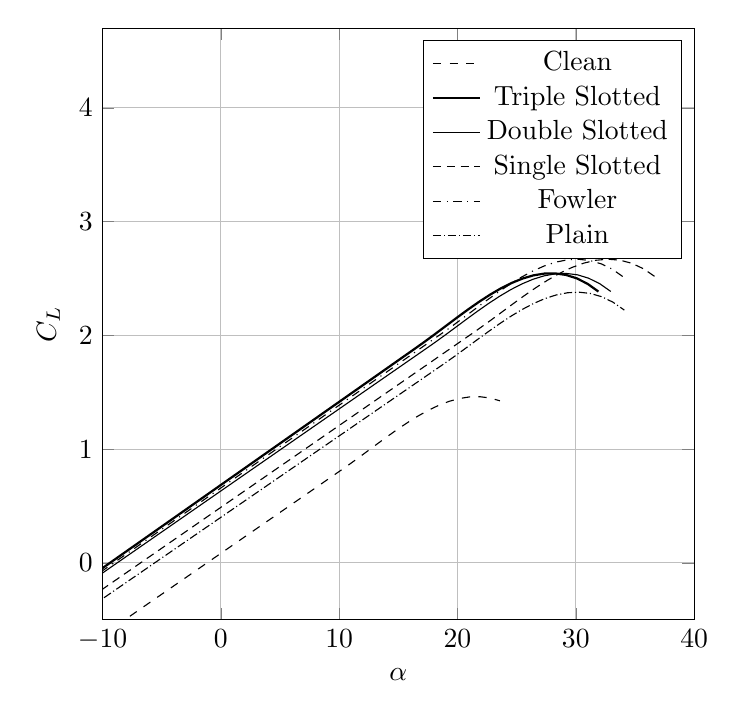
\begin{tikzpicture}

\begin{axis}[
width=0.75\textwidth,
height=0.75\textwidth,
scaled ticks=false, tick label style={/pgf/number format/fixed},
xmin=-10,
xmax=40,
xlabel={$\alpha$},
xmajorgrids,
ymin=-0.5,
ymax=4.7,
ylabel={$C_L$},
ymajorgrids,
legend entries = {Clean\\Triple Slotted\\Double Slotted\\Single Slotted\\Fowler\\Plain\\}]

\addplot [
color=black,
dashed
]
table[row sep=crcr]{
-10.0	-0.6352658757762881\\
-9.138747533153515	-0.5733141304422674\\
-8.27749506630703	-0.5113623851082468\\
-7.416242599460545	-0.4494106397742259\\
-6.55499013261406	-0.38745889444020537\\
-5.693737665767576	-0.3255071491061846\\
-4.832485198921091	-0.26355540377216397\\
-3.9712327320746064	-0.20160365843814332\\
-3.1099802652281214	-0.13965191310412253\\
-2.2487277983816365	-0.0777001677701018\\
-1.3874753315351516	-0.015748422436081128\\
-0.5262228646886667	0.04620332289793959\\
0.3350296021578181	0.1081550682319603\\
1.1962820690043028	0.170106813565981\\
2.0575345358507877	0.2320585589000017\\
2.9187870026972726	0.2940103042340224\\
3.7800394695437576	0.35596204956804306\\
4.6412919363902425	0.4179137949020638\\
5.502544403236727	0.4798655402360845\\
6.3637968700832115	0.5418172855701053\\
7.225049336929696	0.6037690309041259\\
8.08630180377618	0.6657207762381466\\
8.947554270622666	0.7276725215721672\\
9.808806737469151	0.7896242669061881\\
10.670059204315637	0.8518371764996678\\
11.531311671162122	0.9162438895867622\\
12.392564138008607	0.9822400768700835\\
13.253816604855093	1.0485942706393496\\
14.115069071701578	1.1140750031842797\\
14.976321538548063	1.1774508067945915\\
15.837574005394549	1.2374902137600041\\
16.698826472241034	1.2929617563702362\\
17.560078939087518	1.3426339669150065\\
18.421331405934	1.385275377684033\\
19.282583872780485	1.4196545209670353\\
20.14383633962697	1.4445399290537297\\
21.005088806473452	1.4587001342338382\\
21.866341273319936	1.4609036687970764\\
22.72759374016642	1.4499190650331637\\
23.588846207012903	1.4245148552318199\\
};

\addplot [
color=black,
thick
]
table[row sep=crcr]{
-13.0	-0.26471729340342076\\
-12.08342596402438	-0.19775658131163865\\
-11.16685192804876	-0.13079586921985664\\
-10.250277892073141	-0.06383515712807453\\
-9.333703856097522	0.0031255549637075886\\
-8.417129820121902	0.07008626705548959\\
-7.500555784146282	0.1370469791472717\\
-6.583981748170663	0.20400769123905388\\
-5.667407712195043	0.27096840333083594\\
-4.750833676219424	0.33792911542261805\\
-3.834259640243804	0.4048898275144001\\
-2.9176856042681845	0.47185053960618223\\
-2.001111568292565	0.5388112516979643\\
-1.0845375323169453	0.6057719637897464\\
-0.1679634963413258	0.6727326758815285\\
0.7486105396342937	0.7396933879733105\\
1.665184575609913	0.8066541000650926\\
2.5817586115855327	0.8736148121568746\\
3.4983326475611523	0.9405755242486568\\
4.414906683536771	1.0075362363404388\\
5.331480719512391	1.074496948432221\\
6.248054755488011	1.141457660524003\\
7.16462879146363	1.208418372615785\\
8.081202827439249	1.2753790847075672\\
8.997776863414868	1.3423397967993491\\
9.914350899390488	1.4093005088911315\\
10.830924935366108	1.4762612209829133\\
11.747498971341727	1.5432219330746955\\
12.664073007317347	1.6101826451664776\\
13.580647043292966	1.6771433572582595\\
14.497221079268586	1.7441040693500414\\
15.413795115244206	1.8110647814418237\\
16.330369151219823	1.8780254935336056\\
17.24694318719544	1.9457429346696347\\
18.16351722317106	2.0160514914549474\\
19.080091259146677	2.0876763179934232\\
19.996665295122295	2.1591107771941327\\
20.913239331097913	2.22884823196615\\
21.82981336707353	2.295382045218546\\
22.746387403049148	2.3572055798603926\\
23.662961439024766	2.412812198800762\\
24.579535475000384	2.4606952649487277\\
25.496109510976	2.499348141213361\\
26.41268354695162	2.527264190503734\\
27.329257582927237	2.54293677572892\\
28.245831618902855	2.5448592597979895\\
29.162405654878473	2.5315250056200145\\
30.07897969085409	2.5014273761040715\\
30.99555372682971	2.453059734159225\\
31.912127762805355	2.3849154426945485\\
};

\addplot [
color=black,
solid
]
table[row sep=crcr]{
-13.0	-0.305284422992253\\
-12.06212405360256	-0.23763902367190548\\
-11.12424810720512	-0.16999362435155807\\
-10.186372160807679	-0.10234822503121044\\
-9.248496214410238	-0.034702825710862806\\
-8.310620268012798	0.032942573609484826\\
-7.372744321615357	0.10058797292983224\\
-6.434868375217917	0.1682333722501798\\
-5.496992428820477	0.23587877157052745\\
-4.559116482423036	0.3035241708908751\\
-3.621240536025596	0.3711695702112226\\
-2.683364589628156	0.43881496953157006\\
-1.7454886432307162	0.5064603688519176\\
-0.8076126968332761	0.5741057681722651\\
0.13026324956416402	0.6417511674926127\\
1.0681391959616042	0.7093965668129603\\
2.006015142359044	0.7770419661333078\\
2.943891088756484	0.8446873654536553\\
3.881767035153924	0.9123327647740029\\
4.819642981551365	0.9799781640943503\\
5.757518927948805	1.0476235634146978\\
6.6953948743462455	1.1152689627350454\\
7.633270820743686	1.182914362055393\\
8.571146767141126	1.2505597613757407\\
9.509022713538567	1.3182051606960883\\
10.446898659936007	1.385850560016436\\
11.384774606333448	1.4534959593367833\\
12.322650552730888	1.5211413586571307\\
13.260526499128328	1.5887867579774784\\
14.198402445525769	1.656432157297826\\
15.13627839192321	1.7240775566181736\\
16.07415433832065	1.7917229559385208\\
17.01203028471809	1.8593683552588685\\
17.94990623111553	1.9271632014737534\\
18.88778217751297	1.9973356176553976\\
19.82565812391041	2.0694114192644824\\
20.763534070307852	2.1417970328098583\\
21.701410016705292	2.2128988848003743\\
22.639285963102733	2.2811234017448836\\
23.577161909500173	2.3448770101522305\\
24.515037855897614	2.40256613653127\\
25.452913802295054	2.452597207390851\\
26.390789748692494	2.4933766492398233\\
27.328665695089935	2.523310888587039\\
28.266541641487375	2.5408063519413435\\
29.204417587884816	2.5442694658115883\\
30.142293534282256	2.5321066567066293\\
31.080169480679697	2.5027243511353134\\
32.01804542707713	2.454528975606486\\
32.95592137347457	2.385926956628998\\
};

\addplot [
color=black,
densely dashed
]
table[row sep=crcr]{
-13.0	-0.44677435381209774\\
-11.984479254757014	-0.37371932136543284\\
-10.968958509514028	-0.30066428891876795\\
-9.953437764271042	-0.22760925647210295\\
-8.937917019028056	-0.15455422402543806\\
-7.92239627378507	-0.08149919157877317\\
-6.906875528542084	-0.008444159132108331\\
-5.891354783299098	0.06461087331455667\\
-4.875834038056112	0.13766590576122162\\
-3.8603132928131263	0.2107209382078865\\
-2.8447925475701403	0.2837759706545514\\
-1.8292718023271546	0.3568310031012163\\
-0.8137510570841688	0.4298860355478812\\
0.2017696881588169	0.5029410679945461\\
1.2172904334018027	0.575996100441211\\
2.2328111786447886	0.6490511328878759\\
3.2483319238877746	0.7221061653345408\\
4.2638526691307606	0.7951611977812056\\
5.2793734143737465	0.8682162302278706\\
6.2948941596167325	0.9412712626745354\\
7.3104149048597185	1.0143262951212004\\
8.325935650102704	1.0873813275678654\\
9.34145639534569	1.1604363600145302\\
10.356977140588675	1.233491392461195\\
11.372497885831661	1.30654642490786\\
12.388018631074647	1.3796014573545248\\
13.403539376317633	1.45265648980119\\
14.41906012156062	1.525711522247855\\
15.434580866803605	1.5987665546945196\\
16.45010161204659	1.6718215871411841\\
17.465622357289575	1.7448766195878496\\
18.48114310253256	1.8179316520345141\\
19.496663847775544	1.8909866844811787\\
20.512184593018528	1.9640417169278441\\
21.527705338261512	2.037099697328129\\
22.543226083504496	2.1122519482941264\\
23.55874682874748	2.189925531925714\\
24.574267573990465	2.2681028593721644\\
25.58978831923345	2.344766341782756\\
26.605309064476433	2.4178983903067577\\
27.620829809719417	2.485481416093454\\
28.6363505549624	2.545497830292123\\
29.651871300205386	2.595930044052026\\
30.66739204544837	2.63476046852245\\
31.682912790691354	2.6599715148526775\\
32.69843353593434	2.6695455941919706\\
33.71395428117733	2.6614651176896116\\
34.72947502642032	2.633712496494872\\
35.744995771663305	2.5842701417570373\\
36.7605165169063	2.5111204646253755\\
};

\addplot [
color=black,
dashdotted
]
table[row sep=crcr]{
-13.0	-0.28682989146124616\\
-12.039198256763967	-0.2169434470553815\\
-11.078396513527935	-0.14705700264951715\\
-10.117594770291902	-0.07717055824365238\\
-9.156793027055869	-0.00728411383778782\\
-8.195991283819836	0.06260233056807663\\
-7.235189540583803	0.1324887749739414\\
-6.274387797347769	0.20237521937980607\\
-5.3135860541117355	0.2722616637856707\\
-4.352784310875702	0.34214810819153535\\
-3.391982567639668	0.41203455259739996\\
-2.4311808244036346	0.48192099700326463\\
-1.470379081167601	0.5518074414091292\\
-0.5095773379315673	0.6216938858149939\\
0.4512244053044663	0.6915803302208585\\
1.4120261485405	0.7614667746267232\\
2.3728278917765335	0.8313532190325879\\
3.333629635012567	0.9012396634384525\\
4.294431378248601	0.9711261078443172\\
5.255233121484634	1.0410125522501816\\
6.216034864720668	1.1108989966560463\\
7.176836607956702	1.1807854410619112\\
8.137638351192734	1.2506718854677756\\
9.098440094428767	1.32055832987364\\
10.0592418376648	1.390444774279505\\
11.020043580900833	1.4603312186853694\\
11.980845324136865	1.5302176630912339\\
12.941647067372898	1.6001041074970983\\
13.90244881060893	1.6699905519029632\\
14.863250553844964	1.7398769963088276\\
15.824052297080996	1.809763440714692\\
16.78485404031703	1.879649885120557\\
17.74565578355306	1.9495363295264214\\
18.706457526789094	2.019422773932286\\
19.667259270025127	2.0907659633657154\\
20.62806101326116	2.1647172336433034\\
21.588862756497193	2.23957342053901\\
22.549664499733225	2.313606728721447\\
23.510466242969258	2.385089362859226\\
24.47126798620529	2.4522935276209603\\
25.432069729441324	2.5134914276752633\\
26.392871472677356	2.5669552676907514\\
27.35367321591339	2.610957252336032\\
28.314474959149422	2.643769586279719\\
29.275276702385455	2.66366447419043\\
30.236078445621487	2.668914120736771\\
31.19688018885752	2.6577907305873563\\
32.15768193209355	2.628566508410797\\
33.118483675329585	2.5795136588757153\\
34.07928541856565	2.5089043866507144\\
};

\addplot [
color=black,
densely dashdotted
]
table[row sep=crcr]{
-13.0	-0.5298322787040721\\
-12.038770660390707	-0.461043332124695\\
-11.077541320781414	-0.3922543855453177\\
-10.116311981172121	-0.32346543896594054\\
-9.155082641562828	-0.25467649238656304\\
-8.193853301953535	-0.18588754580718586\\
-7.232623962344243	-0.11709859922780869\\
-6.271394622734951	-0.04830965264843157\\
-5.3101652831256585	0.020479293930945663\\
-4.348935943516366	0.0892682405103229\\
-3.387706603907074	0.1580571870897001\\
-2.426477264297781	0.22684613366907735\\
-1.4652479246884886	0.29563508024845453\\
-0.5040185850791962	0.36442402682783176\\
0.4572107545300963	0.433212973407209\\
1.4184400941393887	0.5020019199865862\\
2.3796694337486812	0.5707908665659633\\
3.340898773357974	0.6395798131453406\\
4.302128112967266	0.7083687597247178\\
5.2633574525765585	0.7771577063040951\\
6.224586792185851	0.8459466528834723\\
7.185816131795143	0.9147355994628494\\
8.147045471404436	0.9835245460422268\\
9.108274811013729	1.052313492621604\\
10.069504150623022	1.1211024392009812\\
11.030733490232315	1.1898913857803584\\
11.991962829841608	1.258680332359736\\
12.953192169450901	1.327469278939113\\
13.914421509060194	1.3962582255184903\\
14.875650848669487	1.4650471720978673\\
15.83688018827878	1.533836118677245\\
16.798109527888073	1.6026250652566219\\
17.759338867497366	1.6714140118359992\\
18.72056820710666	1.7402029584153766\\
19.681797546715952	1.8104052485459032\\
20.643026886325245	1.8831838474765048\\
21.604256225934538	1.956864146151692\\
22.56548556554383	2.0297439693214976\\
23.526714905153124	2.100121141735947\\
24.487944244762417	2.166293488145077\\
25.44917358437171	2.226558833298917\\
26.410402923981003	2.279215001947496\\
27.371632263590296	2.322559818840845\\
28.33286160319959	2.3548911087289968\\
29.294090942808882	2.374506696361986\\
30.255320282418175	2.3797044064898403\\
31.21654962202747	2.368782063862583\\
32.17777896163676	2.34003749323026\\
33.13900830124605	2.291768519342898\\
34.10023764085533	2.2222729669505243\\
};
\end{axis}
\end{tikzpicture}%

\caption{Effects of different trailing edge devices upon the lift curve of the B747-100B with $\delta_f=\SI{30}{\degree}$, $\frac{c_f}{c}=0.18$ and $\delta_s=\SI{15}{\degree}$}
\end{figure}
%
\begin{figure}[H]
\centering
%CL alpha high lift WING
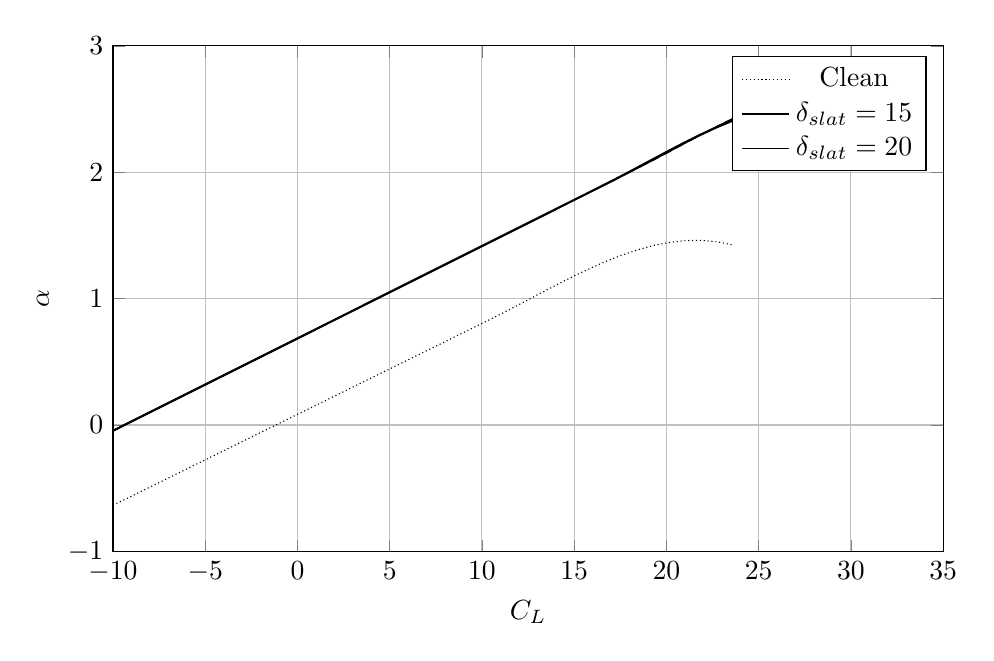
\begin{tikzpicture}

\begin{axis}[
width=\textwidth,
height=0.66\textwidth,
scaled ticks=false, tick label style={/pgf/number format/fixed},
xmin=-10,
xmax=35,
xlabel={$C_L$},
xmajorgrids,
ymin=-1,
ymax=3,
ylabel={$\alpha$},
ymajorgrids,
legend entries = {Clean\\$\delta_{\text{slat}}=\SI{15}{\degree}$\\$\delta_{\text{slat}}=\SI{20}{\degree}$\\}]

\addplot [
color=black,
densely dotted
]
table[row sep=crcr]{
-10.0	-0.6352658757762881\\
-9.138747533153515	-0.5733141304422674\\
-8.27749506630703	-0.5113623851082468\\
-7.416242599460545	-0.4494106397742259\\
-6.55499013261406	-0.38745889444020537\\
-5.693737665767576	-0.3255071491061846\\
-4.832485198921091	-0.26355540377216397\\
-3.9712327320746064	-0.20160365843814332\\
-3.1099802652281214	-0.13965191310412253\\
-2.2487277983816365	-0.0777001677701018\\
-1.3874753315351516	-0.015748422436081128\\
-0.5262228646886667	0.04620332289793959\\
0.3350296021578181	0.1081550682319603\\
1.1962820690043028	0.170106813565981\\
2.0575345358507877	0.2320585589000017\\
2.9187870026972726	0.2940103042340224\\
3.7800394695437576	0.35596204956804306\\
4.6412919363902425	0.4179137949020638\\
5.502544403236727	0.4798655402360845\\
6.3637968700832115	0.5418172855701053\\
7.225049336929696	0.6037690309041259\\
8.08630180377618	0.6657207762381466\\
8.947554270622666	0.7276725215721672\\
9.808806737469151	0.7896242669061881\\
10.670059204315637	0.8518371764996678\\
11.531311671162122	0.9162438895867622\\
12.392564138008607	0.9822400768700835\\
13.253816604855093	1.0485942706393496\\
14.115069071701578	1.1140750031842797\\
14.976321538548063	1.1774508067945915\\
15.837574005394549	1.2374902137600041\\
16.698826472241034	1.2929617563702362\\
17.560078939087518	1.3426339669150065\\
18.421331405934	1.385275377684033\\
19.282583872780485	1.4196545209670353\\
20.14383633962697	1.4445399290537297\\
21.005088806473452	1.4587001342338382\\
21.866341273319936	1.4609036687970764\\
22.72759374016642	1.4499190650331637\\
23.588846207012903	1.4245148552318199\\
};

\addplot [
color=black,
thick
]
table[row sep=crcr]{
-13.0	-0.26471729340342076\\
-12.08342596402438	-0.19775658131163865\\
-11.16685192804876	-0.13079586921985664\\
-10.250277892073141	-0.06383515712807453\\
-9.333703856097522	0.0031255549637075886\\
-8.417129820121902	0.07008626705548959\\
-7.500555784146282	0.1370469791472717\\
-6.583981748170663	0.20400769123905388\\
-5.667407712195043	0.27096840333083594\\
-4.750833676219424	0.33792911542261805\\
-3.834259640243804	0.4048898275144001\\
-2.9176856042681845	0.47185053960618223\\
-2.001111568292565	0.5388112516979643\\
-1.0845375323169453	0.6057719637897464\\
-0.1679634963413258	0.6727326758815285\\
0.7486105396342937	0.7396933879733105\\
1.665184575609913	0.8066541000650926\\
2.5817586115855327	0.8736148121568746\\
3.4983326475611523	0.9405755242486568\\
4.414906683536771	1.0075362363404388\\
5.331480719512391	1.074496948432221\\
6.248054755488011	1.141457660524003\\
7.16462879146363	1.208418372615785\\
8.081202827439249	1.2753790847075672\\
8.997776863414868	1.3423397967993491\\
9.914350899390488	1.4093005088911315\\
10.830924935366108	1.4762612209829133\\
11.747498971341727	1.5432219330746955\\
12.664073007317347	1.6101826451664776\\
13.580647043292966	1.6771433572582595\\
14.497221079268586	1.7441040693500414\\
15.413795115244206	1.8110647814418237\\
16.330369151219823	1.8780254935336056\\
17.24694318719544	1.9457429346696347\\
18.16351722317106	2.0160514914549474\\
19.080091259146677	2.0876763179934232\\
19.996665295122295	2.1591107771941327\\
20.913239331097913	2.22884823196615\\
21.82981336707353	2.295382045218546\\
22.746387403049148	2.3572055798603926\\
23.662961439024766	2.412812198800762\\
24.579535475000384	2.4606952649487277\\
25.496109510976	2.499348141213361\\
26.41268354695162	2.527264190503734\\
27.329257582927237	2.54293677572892\\
28.245831618902855	2.5448592597979895\\
29.162405654878473	2.5315250056200145\\
30.07897969085409	2.5014273761040715\\
30.99555372682971	2.453059734159225\\
31.912127762805355	2.3849154426945485\\
};

\addplot [
color=black,
solid
]
table[row sep=crcr]{
-13.0	-0.26471729340342076\\
-12.050290618674005	-0.1953358643449984\\
-11.10058123734801	-0.1259544352865758\\
-10.150871856022015	-0.0565730062281532\\
-9.20116247469602	0.012808422830269173\\
-8.251453093370024	0.08218985188869177\\
-7.301743712044028	0.15157128094711436\\
-6.352034330718032	0.2209527100055369\\
-5.402324949392036	0.2903341390639595\\
-4.45261556806604	0.3597155681223821\\
-3.502906186740044	0.4290969971808046\\
-2.553196805414048	0.4984784262392272\\
-1.6034874240880521	0.5678598552976497\\
-0.6537780427620562	0.6372412843560723\\
0.2959313385639397	0.7066227134144949\\
1.2456407198899355	0.7760041424729175\\
2.1953501012159315	0.8453855715313401\\
3.1450594825419276	0.9147670005897626\\
4.094768863867923	0.9841484296481852\\
5.044478245193919	1.0535298587066078\\
5.994187626519915	1.1229112877650302\\
6.943897007845911	1.1922927168234527\\
7.893606389171907	1.2616741458818752\\
8.843315770497902	1.331055574940298\\
9.793025151823898	1.4004370039987202\\
10.742734533149893	1.4698184330571429\\
11.692443914475888	1.5391998621155656\\
12.642153295801883	1.608581291173988\\
13.591862677127878	1.6779627202324106\\
14.541572058453873	1.747344149290833\\
15.491281439779868	1.8167255783492555\\
16.440990821105864	1.886107007407678\\
17.39070020243186	1.9554884364661\\
18.340409583757854	2.0248821249799214\\
19.29011896508385	2.0962807467533686\\
20.239828346409844	2.169969366229889\\
21.18953772773584	2.2442720300580845\\
22.139247109061834	2.3175127848865547\\
23.08895649038783	2.388015677363901\\
24.038665871713825	2.454104754138723\\
24.98837525303982	2.514104061859621\\
25.938084634365815	2.566337647175195\\
26.88779401569181	2.6091295567340493\\
27.837503397017805	2.6408038371847793\\
28.7872127783438	2.6596845351759866\\
29.736922159669795	2.664095697356278\\
30.68663154099579	2.6523613703742432\\
31.636340922321786	2.6228056008784906\\
32.58605030364778	2.5737524355176165\\
33.5357596849738	2.5035259209402225\\
};

\addplot [
color=black,
densely dashed
]
table[row sep=crcr]{
-13.0	-0.26471729340342076\\
-12.042787039079508	-0.19478768709671956\\
-11.085574078159016	-0.12485808079001803\\
-10.128361117238525	-0.054928474483316836\\
-9.171148156318033	0.015001131823384362\\
-8.213935195397541	0.08493073813008556\\
-7.256722234477049	0.15486034443678676\\
-6.299509273556557	0.22478995074348795\\
-5.342296312636066	0.2947195570501893\\
-4.385083351715574	0.3646491633568905\\
-3.4278703907950816	0.4345787696635918\\
-2.4706574298745894	0.5045083759702931\\
-1.5134444689540971	0.5744379822769944\\
-0.5562315080336049	0.6443675885836957\\
0.40098145288688736	0.714297194890397\\
1.3581944138073796	0.7842268011970983\\
2.315407374727872	0.8541564075037995\\
3.272620335648364	0.9240860138105008\\
4.229833296568856	0.994015620117202\\
5.187046257489348	1.0639452264239033\\
6.1442592184098395	1.1338748327306045\\
7.101472179330331	1.203804439037306\\
8.058685140250823	1.273734045344007\\
9.015898101171315	1.3436636516507083\\
9.973111062091807	1.4135932579574095\\
10.930324023012298	1.4835228642641107\\
11.88753698393279	1.5534524705708121\\
12.844749944853282	1.6233820768775133\\
13.801962905773774	1.6933116831842145\\
14.759175866694266	1.763241289490916\\
15.716388827614757	1.833170895797617\\
16.67360178853525	1.9031005021043184\\
17.630814749455745	1.9730301084110198\\
18.588027710376238	2.042959714717721\\
19.54524067129673	2.114527416203136\\
20.502453632217225	2.1886182708619764\\
21.45966659313772	2.263521177009215\\
22.416879554058212	2.3375201564251347\\
23.374092514978706	2.4088992308900172\\
24.3313054758992	2.47594242218414\\
25.288518436819693	2.536933752087789\\
26.245731397740187	2.590157242381241\\
27.20294435866068	2.633896914844782\\
28.160157319581174	2.666436791258689\\
29.117370280501667	2.6860608934032433\\
30.07458324142216	2.6910532430587297\\
31.031796202342655	2.6796978620054306\\
31.989009163263148	2.650278772023621\\
32.94622212418364	2.601079994893582\\
33.90343508510412	2.5303855523955994\\
};

\addplot [
color=black,
dashdotted
]
table[row sep=crcr]{
-13.0	-0.26471729340342076\\
-12.059380489914654	-0.1959999288146499\\
-11.118760979829307	-0.1272825642258787\\
-10.178141469743961	-0.0585651996371076\\
-9.237521959658615	0.01015216495166349\\
-8.296902449573269	0.07886952954043436\\
-7.356282939487922	0.14758689412920545\\
-6.415663429402576	0.21630425871797648\\
-5.47504391931723	0.2850216233067476\\
-4.5344244092318835	0.3537389878955186\\
-3.5938048991465372	0.4224563524842896\\
-2.653185389061191	0.4911737170730607\\
-1.7125658789758444	0.5598910816618317\\
-0.771946368890498	0.6286084462506027\\
0.16867314119484855	0.6973258108393737\\
1.109292651280195	0.7660431754281448\\
2.0499121613655413	0.8347605400169158\\
2.9905316714508876	0.9034779046056869\\
3.931151181536234	0.972195269194458\\
4.87177069162158	1.0409126337832288\\
5.812390201706926	1.1096299983720002\\
6.753009711792273	1.178347362960771\\
7.693629221877619	1.2470647275495421\\
8.634248731962966	1.315782092138313\\
9.574868242048312	1.384499456727084\\
10.515487752133659	1.4532168213158552\\
11.456107262219005	1.5219341859046263\\
12.396726772304351	1.5906515504933973\\
13.337346282389698	1.6593689150821684\\
14.277965792475044	1.728086279670939\\
15.21858530256039	1.7968036442597102\\
16.159204812645736	1.8655210088484813\\
17.099824322731084	1.9342383734372524\\
18.040443832816432	2.003061516867686\\
18.98106334290178	2.0742194920985826\\
19.92168285298713	2.1473878885393463\\
20.862302363072477	2.220938399712569\\
21.802921873157825	2.2932427191408378\\
22.743541383243173	2.3626725403467503\\
23.68416089332852	2.427599556852888\\
24.62478040341387	2.4863954621818483\\
25.565399913499217	2.53743194985622\\
26.506019423584565	2.579080713398592\\
27.446638933669913	2.6097134463315568\\
28.38725844375526	2.627701842177701\\
29.32787795384061	2.631417594459621\\
30.268497463925957	2.619232396699906\\
31.209116974011305	2.5895179424211383\\
32.14973648409665	2.5406459251459195\\
33.09035599418198	2.470988038396837\\
};
\end{axis}
\end{tikzpicture}%

\caption{Effects of different $\delta_s$ upon the lift curve of the B747-100B with $\delta_f=\SI{30}{\degree}$, $\frac{c_f}{c}=0.18$ and Triple slotted flaps}
\label{fig:SlatSensibility}
\end{figure}
%
\noindent
As can be seen the code is able to manage different high lift devices settings with good results; for example the more the flap is deflected, the more the $C_{L\text{max}}$ grows; also the effect of the $\frac{c_f}{c}$ ratio is modeled well, in fact, more flap chord allows to achieve higher $C_{L\text{max}}$. Finally it has to be noted the effect of slats deflection; the latter, in fact, influences not only the $C_{L\text{max}}$ but also the $\alpha_{\text{stall}}$ increasing them when the deflection is bigger. This effect becomes gradually smaller with increasing slats deflection becoming null, and then negative, for slats deflection angles between 25° and 30°, as shown in figure \ref{fig:SlatSensibility}.